% interactcadsample.tex
% v1.03 - April 2017

\documentclass[]{interact}

\usepackage{epstopdf}% To incorporate .eps illustrations using PDFLaTeX, etc.
\usepackage{subfigure}% Support for small, `sub' figures and tables
%\usepackage[nolists,tablesfirst]{endfloat}% To `separate' figures and tables from text if required

\usepackage{natbib}% Citation support using natbib.sty
\bibpunct[, ]{(}{)}{;}{a}{}{,}% Citation support using natbib.sty
\renewcommand\bibfont{\fontsize{10}{12}\selectfont}% Bibliography support using natbib.sty

\theoremstyle{plain}% Theorem-like structures provided by amsthm.sty
\newtheorem{theorem}{Theorem}[section]
\newtheorem{lemma}[theorem]{Lemma}
\newtheorem{corollary}[theorem]{Corollary}
\newtheorem{proposition}[theorem]{Proposition}

\theoremstyle{definition}
\newtheorem{definition}[theorem]{Definition}
\newtheorem{example}[theorem]{Example}

\theoremstyle{remark}
\newtheorem{remark}{Remark}
\newtheorem{notation}{Notation}


% tightlist command for lists without linebreak
\providecommand{\tightlist}{%
  \setlength{\itemsep}{0pt}\setlength{\parskip}{0pt}}



\usepackage{hyperref}
\usepackage[utf8]{inputenc}
\def\tightlist{}
\usepackage{setspace}
\usepackage{graphicx}
\usepackage{nicematrix}
\NiceMatrixOptions{code-for-first-row = \color{red} ,code-for-last-row = \color{red} ,code-for-first-col = \color{blue} ,code-for-last-col = \color{blue}}


\begin{document}


\articletype{Short Technical Note}

\title{New and simplified manual controls for projection and slice
tours, with application to exploring classification boundaries in high
dimensions}


\author{\name{Ursula Laa$^{a}$, Alex Aumann$^{b}$, Dianne
Cook$^{c}$, German Valencia$^{b}$}
\affil{$^{a}$Institute of Statistics, University of Natural Resources
and Life Sciences, Vienna; $^{b}$School of Physics and Astronomy, Monash
University; $^{c}$Department of Econometrics and Business Statistics,
Monash University}
}

\thanks{CONTACT Ursula
Laa. Email: \href{mailto:ursula.laa@boku.ac.at}{\nolinkurl{ursula.laa@boku.ac.at}}, Alex
Aumann. Email: \href{mailto:aaum0002@student.monash.edu}{\nolinkurl{aaum0002@student.monash.edu}}, Dianne
Cook. Email: \href{mailto:dicook@monash.edu}{\nolinkurl{dicook@monash.edu}}, German
Valencia. Email: \href{mailto:german.valencia@monash.edu}{\nolinkurl{german.valencia@monash.edu}}}

\maketitle

\begin{abstract}
This paper describes new user controls for examining high-dimensional
data using low-dimensional linear projections and slices. A user can
interactively change the coefficients of a variable in a low-dimensional
projection, which is useful for exploring the sensitivity of structure
to particular variables. The user can also interactively shift the slice
center, which is useful for exploring how structure changes in local
subspaces. These controls are implemented in Mathematica to take
advantage of it's mathematics functions, and interactivity tools that
allow construction of functions that interact with the position of the
cursor. We demonstrate the usefulness of this new tool with an example
exploring region boundaries in classification problems.
\end{abstract}

\begin{keywords}
data visualisation; grand tour; statistical computing; statistical
graphics; multivariate data; dynamic graphics
\end{keywords}

\hypertarget{introduction}{%
\section{Introduction}\label{introduction}}

From a statistical perspective 3D is a rare data dimension, so unlike in
most 3D rotation computer graphics applications, the more useful methods
for data analysis need to work for arbitrary dimension. A good approah
is to show projections from an arbitrary dimensional space to create
dynamic data visualizations called \emph{tours}. Tours involve views of
high-dimensional (\(p\)) data with low-dimensional (\(d\)) projections.
In his original paper on the grand tour, \citet{As85} provided several
algorithms for tour paths that could theoretically show the viewer the
data \emph{from all sides}. Prior to Asimov's work, there were numerous
preparatory developments including \citet{tukey}'s PRIM-9. PRIM-9 had
user-controlled rotations on coordinate axes, allowing one to manually
tour through low-dimensional projections. (A video illustrating the
capabilities is available through video library of \citet{ASA22}.)
Steering through all possible projections is impossible, unlike Asimov's
tours which allows one to quickly see many, many different projections.
After Asimov there have been many, many tour developments, which are
summarized in \citet{lee2021}.

One such direction of work develops the ideas from PRIM-9, to provide
manual control of a tour. \citet{cook_manual_1997} describe controls for
1D (or 2D) projections, respectively in a 2D (or 3D) manipulation space,
allowing the user to select any variable axis, and rotate it into, or
out of, or around the projection through horizontal, vertical, oblique,
radial or angular changes in value. \citet{spyrison_spinifex_2020}
refined this algorithm and implemented it to generate radial tour
animation sequences.

Manual controls are especially useful for assessing sensitivity of
structure to particular elements of the projection. There are many
places where it is useful. In exploratory data analysis, where one sees
clusters in a projection, can some variables be removed from the
projection without affecting the clustering. For interpreting models,
one can reduce or increase a variable's contribution to examine the
variable importance. Having the user interact with a projection is
extremely valuable for understanding high-dimensional data. However,
these algorithms have two problems: (1) the pre-processing of creating a
manipulation space overly complicates the algorithm, (2) extending to
higher dimensional control is difficult.

Another potentially useful manual control, is to allow the user to
control the position of the center of a slice. The slice tour was
introduced in \citet{slicetour}. It operates by converting the
projection plane into a slice, by removing or de-emphasizing points that
are further than a fixed orthogonal distance from the plane. The
projection plane is usually thought of as passing through the center of
the data. Manual control would allow the user to change the value of
center point, by shifting it along a coordinate axis, while keeping the
orientation of the projection plane fixed. The purpose would be to
explore how or if the shape of the data, in the space orthogonal to the
projection, changes as one gets away from the center.

This paper explains the new manual controls for projection and slice
tours. The next section describes the new algorithm for manual control,
for both projections and slices. The use of these methods are
illustrated to compare and contrast boundaries constructed by different
classifiers. The software section describes a mathematica notebook that
is used for the application, and describes the interactive environment
that would be desirable within R as new technology becomes available.
The paper is accompanied by an appendix with more details and
adjustments to the manual controls, and two mathematica notebooks, one
focused on the application, and the other that could be used generically
for new data.

\hypertarget{sec:method}{%
\section{How to construct a manual tour}\label{sec:method}}

A manual tour allows the user to alter the coefficients of one (or more)
variables contributing to a \(d-D\) projection. The initial ingredients
are an orthonormal basis (\(A_{p\times d}\)) defining the projection of
the data, and a variable id (\(m \in \{1, ..., p\}\)) specifying which
coefficient will be changed. A method to update the values of the
component (\(m^{th}\) row of \(A_{p\times d}\)) of the controlled
variable \(V_m\) is then needed.

\hypertarget{existing-methods}{%
\subsection{Existing methods}\label{existing-methods}}

The method for updating component values in \citet{cook_manual_1997}
(and utilised in \citet{spyrison_spinifex_2020}) are prescribed
primarily for a 2D projection, to take advantage of (then) newly
developed 3D trackball controls made available for computer gaming. The
first step was to construct a 3D manipulation space from a 2D
projection. In this space, the coefficient of the controlled variable
ranges between -1 and 1. Movements of a cursor are recorded and
converted into changes in the values of \(V_m\) thus changing the
displayed 2D projection. The algorithm also provided constraints to
horizontal, vertical, radial or angular motions only. The construction
of the manipulation space overly complicates the manual controls,
especially when considering possible techniques that will apply to
arbitrary \(d\).

\hypertarget{a-new-simpler-and-broadly-applicable-approach}{%
\subsection{A new simpler and broadly applicable
approach}\label{a-new-simpler-and-broadly-applicable-approach}}

The new approach emerged from experiments on the tour using the linear
algebra capabilities, and relatively new interactive graphics interface,
available in \citet{Mathematica}. The components corresponding to
\(V_m\) are directly controlled by cursor movement, which updates row
\(m\) of \(A\). The updated matrix is then orthonormalised.

\hypertarget{algorithm}{%
\subsubsection{Algorithm}\label{algorithm}}

\begin{enumerate}
\def\labelenumi{\arabic{enumi}.}
\tightlist
\item
  Provide \(A\), and \(m\). (Note that \(m\) could also be automatically
  chosen as the component that is closest to the cursor position.)
\item
  Change values in row \(m\), for example, if \(d=2\) gives \[
  A^* = [ \boldsymbol{a}^*_1~\boldsymbol{a}^*_2 ] = \left[ \begin{array}{cc} a_{11} & a_{12}\\
                             \vdots & \vdots \\
                             a^*_{m1} & a^*_{m2}\\
                             \vdots & \vdots \\
                             a_{p1} & a_{p2} 
       \end{array}\right].
  \] \noindent A large change in these values would correspond to making
  a large jump from the current projection. Small changes would
  correspond to tracking a cursor, making small jumps from the current
  projection.
\item
  Orthonormalise \(A^*\), using Gram-Schmidt.

  \begin{enumerate}
  \def\labelenumii{\roman{enumii}.}
  \tightlist
  \item
    Normalise \(\boldsymbol{a}^*_1\) and \(\boldsymbol{a}^*_2\).
  \item
    \(\boldsymbol{a}^*_2 = \boldsymbol{a}^*_2 - <\boldsymbol{a}^*_1\cdot\boldsymbol{a}^*_2>\boldsymbol{a}^*_1\).
  \end{enumerate}
\end{enumerate}

This algorithm will produce the changes to a projection as illustrated
in Figure \ref{fig:manualsequence}. The controlled variable, \(V_m\),
corresponds to the black line, and sequential changes to row \(m\) of
\(A\) can be seen to roughly follow a specified position (orange dot).
Changes in the other components happen as a result of the
orthonormalisation, but are uncontrolled.

\begin{figure}
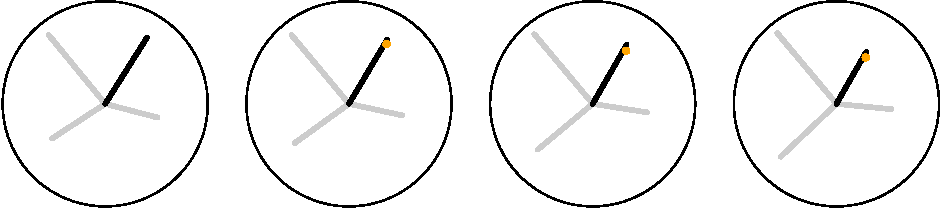
\includegraphics[width=1\linewidth]{paper_files/figure-latex/manualsequence-1} \caption{Sequence of projections where contribution of one variable is controlled (black) is changed using unconstrained orthonormalisation. The dot (orange) indicates the chosen values for the controlled variable. It can be seen that the actual axis does not precisely match the chosen position, but it is close.}\label{fig:manualsequence}
\end{figure}

\hypertarget{refinements-to-enforce-exact-position}{%
\subsection{Refinements to enforce exact
position}\label{refinements-to-enforce-exact-position}}

The problem with new simple method is that it is not faithful to the
precise values for \(V_m\) because the orthonormalisation will change
them. There are numerous ways that this can be enforced, and details are
in the Appendix.

\hypertarget{manual-control-for-slices}{%
\subsection{Manual control for slices}\label{manual-control-for-slices}}

To better explore the space we combine the manual controls for the
projection with manual controls for slicing. A slice is a section of the
data that is defined by a projection, a center point that is anchoring
it in the high-dimensional space and the slice thickness \(h\)
\citep{slicetour}. A data point is inside the slice if its orthogonal
distance from the projection plane (passing through the center point) is
below the thickness \(h\). This orthogonal distance is computed in terms
of the component that is normal on the projection plane. For
\(\mathbf{x}_i\) a \(p\) dimensional data point and \(\mathbf{c}\) the
center point (in the same \(p\) dimensional space) we compute the
orthogonal distance as \begin{equation}
v_i^2 = ||\mathbf{x}_i' - \mathbf{c}'||^2 = \mathbf{x}_i'^2 + \mathbf{c}'^2 - 2 \mathbf{x}_i'\cdot\mathbf{c}' ,
\label{eq:slice}
\end{equation} with
\(\mathbf{c}' = \mathbf{c} - (\mathbf{c}\cdot \mathbf{a}_1) \mathbf{a}_1 - (\mathbf{c}\cdot \mathbf{a}_2 )\mathbf{a}_2\),
\(\mathbf{x}_i' = \mathbf{x}_i - (\mathbf{x}_i\cdot \mathbf{a}_1) \mathbf{a}_1 - (\mathbf{x}_i\cdot \mathbf{a}_2) \mathbf{a}_2\)
and \(\mathbf{a}_k, k=1,2 (=d)\) denoting the columns of the projection
matrix, \(\mathbf{A}=(\mathbf{a}_1, \mathbf{a}_2)\).

\hypertarget{shifting-the-center}{%
\subsubsection{Shifting the center}\label{shifting-the-center}}

In the case of a single orthogonal direction on the projection plane we
can pick a sequence of center points \(\mathbf{c}\) in steps along that
direction to move the slice and fully cover the data space. This no
longer works in higher-dimensional spaces, and we can think of picking
one direction and shifting the slice along the component orthogonal to
the projection plane. In practice we define the center point
\(\mathbf{c}\) explicitly in terms of all \(p\) components and calculate
the slice display following Eq. \ref{eq:slice}.

\hypertarget{changing-the-thickness}{%
\subsubsection{Changing the thickness}\label{changing-the-thickness}}

In addition it is also useful to interactively change the slice
thickness \(h\) (also called the slice radius), in particular to find
the preferred value for exploring the input data. This was implemented
as a slider, and to allow the user to efficiently explore the
interesting range we provide the slider range as an input. For guidance
the estimates of the number of points inside the slice as a function of
the original sample size \(N\) and the number of dimensions \(p\) from
\citet{sectionpursuit} can be used: in case of a uniform distribution
inside a sphere of radius \(R\) a slice with thickness \(h\) will
contain \(N_S\) points, with \begin{equation}
N_S = \frac{N}{2} \left(\frac{h}{R}\right)^{p-2} \left(p - (p-2)\left(\frac{h}{R}\right)^{2}\right).
\label{eq:count}
\end{equation}

\begin{figure}

{\centering 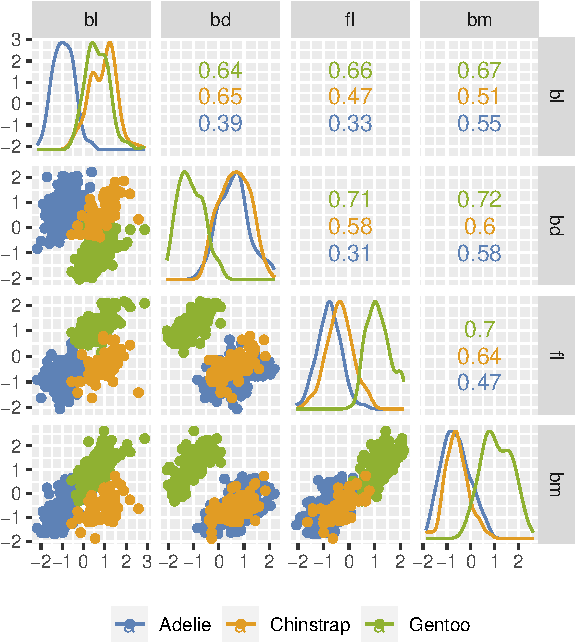
\includegraphics[width=0.8\linewidth]{paper_files/figure-latex/penguins-scatmat-1} 

}

\caption{Scatterplot matrix of the (standardised) penguins data. The three species are reasonably different in size, with Gentoo distinguised from the other two on body depth relative to flipper length and body mass.}\label{fig:penguins-scatmat}
\end{figure}

\hypertarget{sec:examples}{%
\section{Application}\label{sec:examples}}

To illustrate the usefulness of the manual controls we use the 4D
penguins data \citep{penguins} and look at classification models
following \citet{sam11271}. We will show how classification boundaries
can be explored and better understood on projections and slices through
4D space. Figure \ref{fig:penguins-scatmat} shows a scatterplot matrix
of this data. There are four variables
(\texttt{bl\ =\ bill\_length\_mm,\ bd\ =\ bill\_depth\_mm,\ fl\ =\ flipper\_length\_mm,\ bm\ =\ body\_mass\_g})
measuring the size of the penguins from three species (Adelie, Chinstrap
and Gentoo). The scatterplot matrix shows that the three species appear
to be likely separable, and that at least the Gentoo can be
distinguished from the other two species when \texttt{bd} is paired with
\texttt{fl} or \texttt{bm}. The steps for exploring boundaries in this
example are as follows:

\begin{enumerate}
\def\labelenumi{\arabic{enumi}.}
\tightlist
\item
  Build your classification model.
\item
  Predict the class for a dense grid of values covering the data space.
\item
  Examine projections, using a manual tour so that the contribution of
  any variable is controlled.
\item
  Slice through the center, to explore where the boundaries will likely
  meet.
\item
  Move the slice by changing the center in the direction of a single
  variable to explore the extent of a boundary for a single group
  relative to a variable.
\end{enumerate}

\hypertarget{constructing-the-4d-prediction-regions}{%
\subsection{Constructing the 4D prediction
regions}\label{constructing-the-4d-prediction-regions}}

We use the \texttt{classifly} package \citep{classifly} to generate
predictions across the 4D cube spanned by the data, with two
classification models: linear discriminant analysis (LDA) and random
forest (RF). Both the data and the model points in the grid are centered
and scaled (standard deviation \(= 1\)).

\hypertarget{exploring-projections-manually}{%
\subsection{Exploring projections
manually}\label{exploring-projections-manually}}

We start by first exploring the projections of the model prediction.
Figure \ref{proj1} summarises the process. Through manual rotation of
the view we can get a feeling for where in the space we primarily
predict each of the three species, and we also get a sense of the
difference between the two models. To illustrate this difference we have
manually rotated the projection for the RF model (left plot) to identify
a projection that shows the non-linear but block-type structure that is
typical of this type of model. This particular projection (\(A_1\)) is
exported so that the same projection can be used to show the LDA model
(middle plot) and the actual data (right plot). What can be seen is the
linearity of the LDA model, where the boundaries are linear and oblique
to the variable axes. And, interestingly this particular projection of
the original data shows very distinct clusters of the three species.
That means, the obscuring of the boundaries between groups for both of
the models is driven by what is happening in the orthogonal space to the
plane of the selected projection.

\begin{figure*}[ht]
\centerline{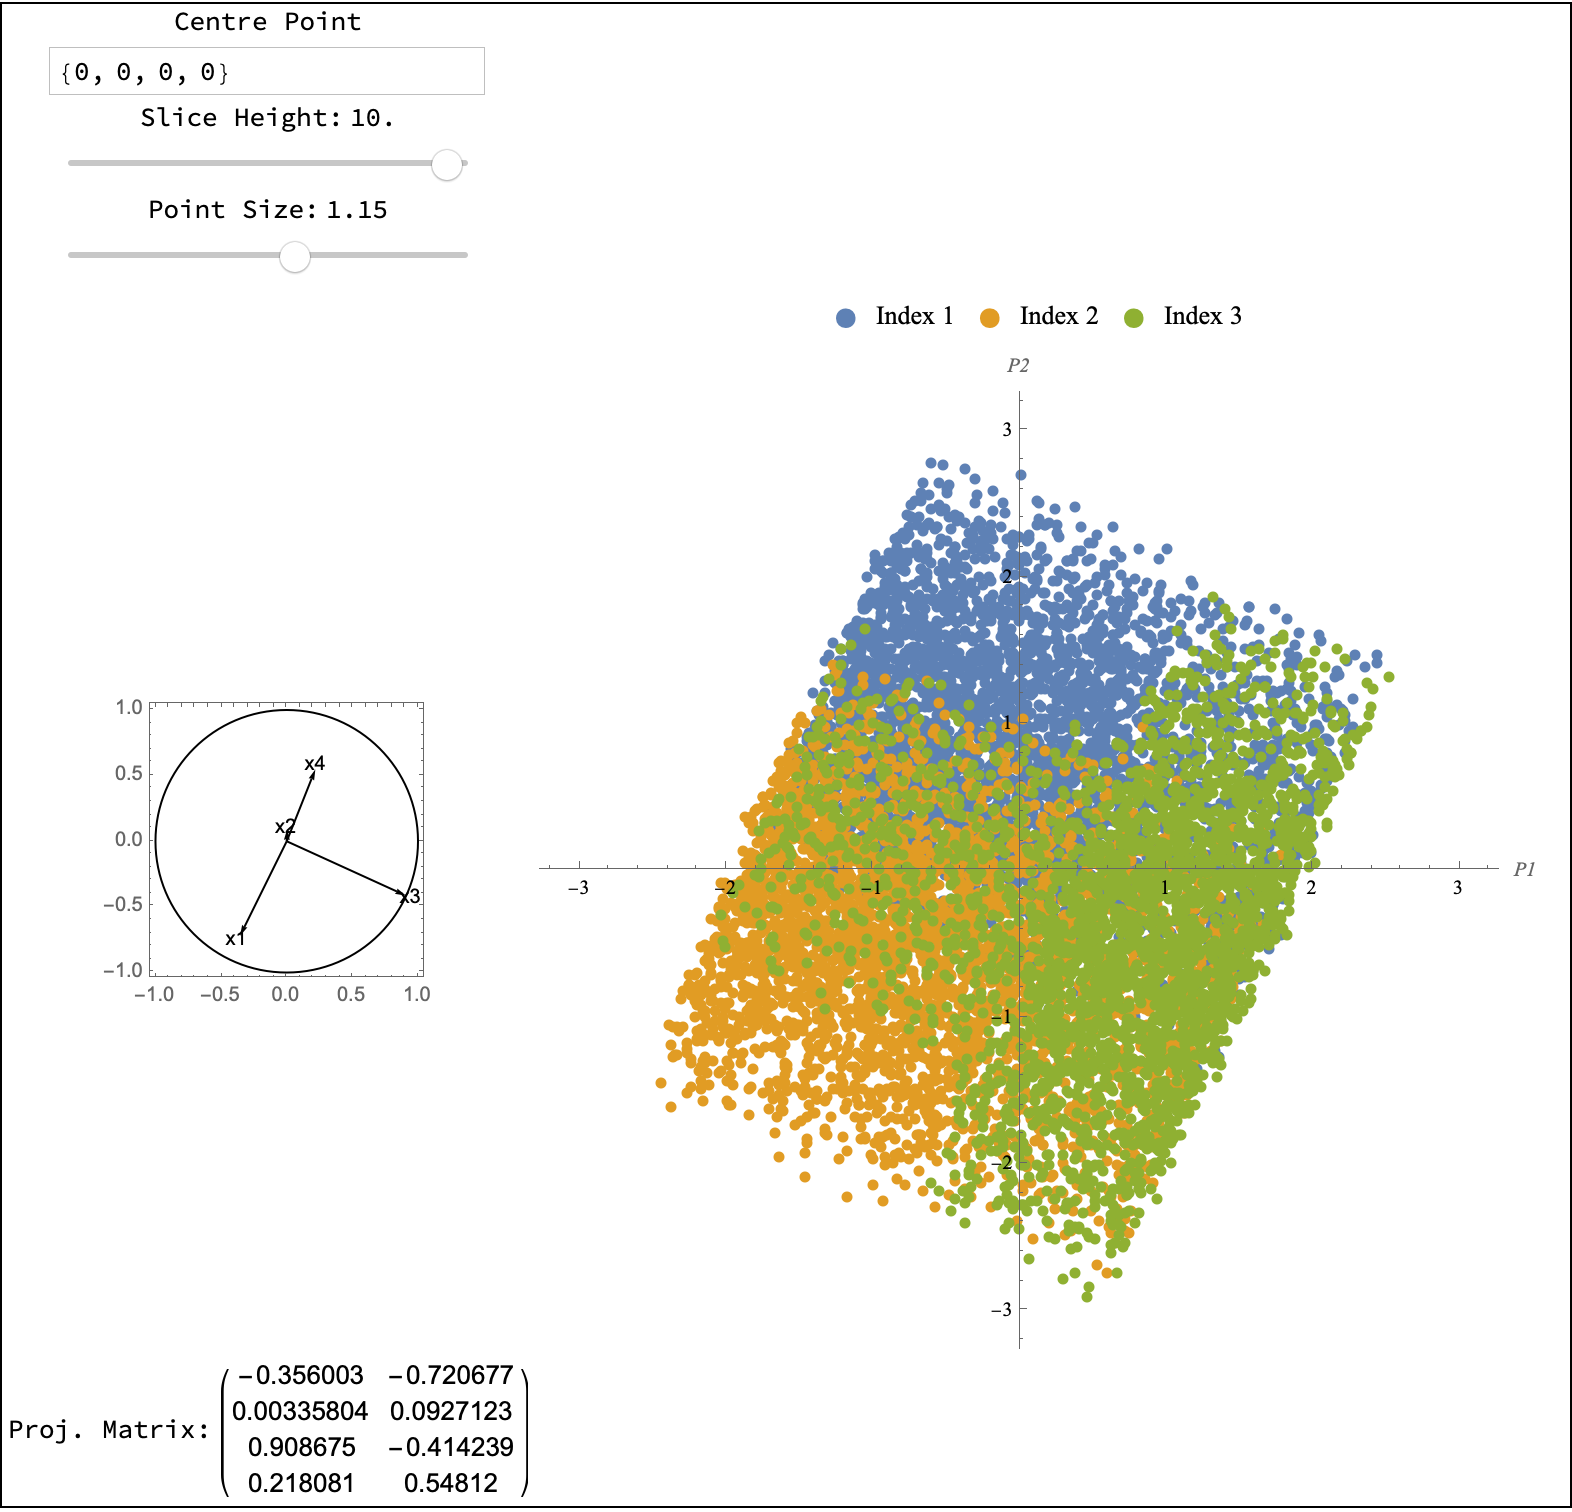
\includegraphics[width=0.32\textwidth]{figures/proj1_rf.png}
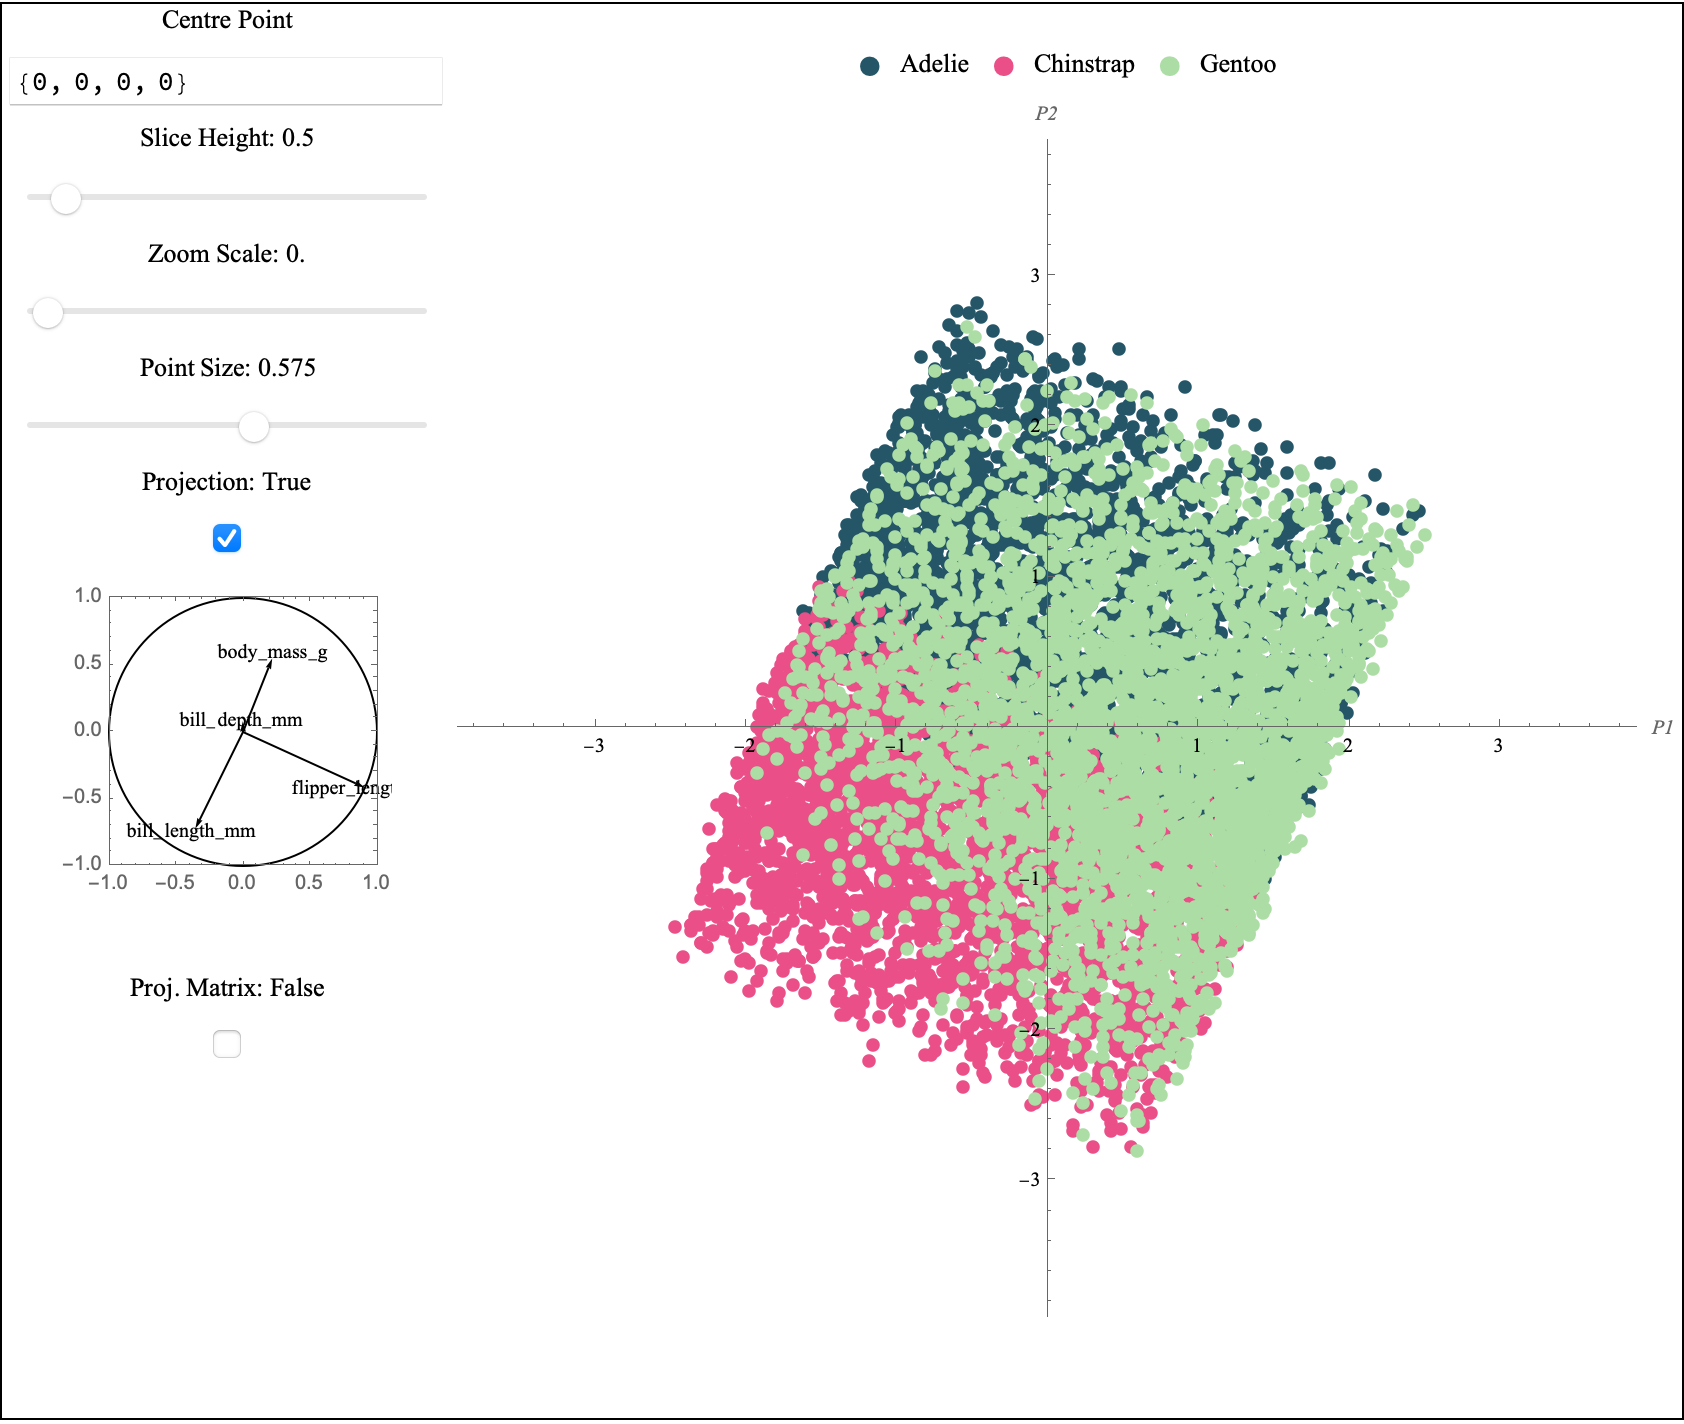
\includegraphics[width=0.32\textwidth]{figures/proj1_lda.png}
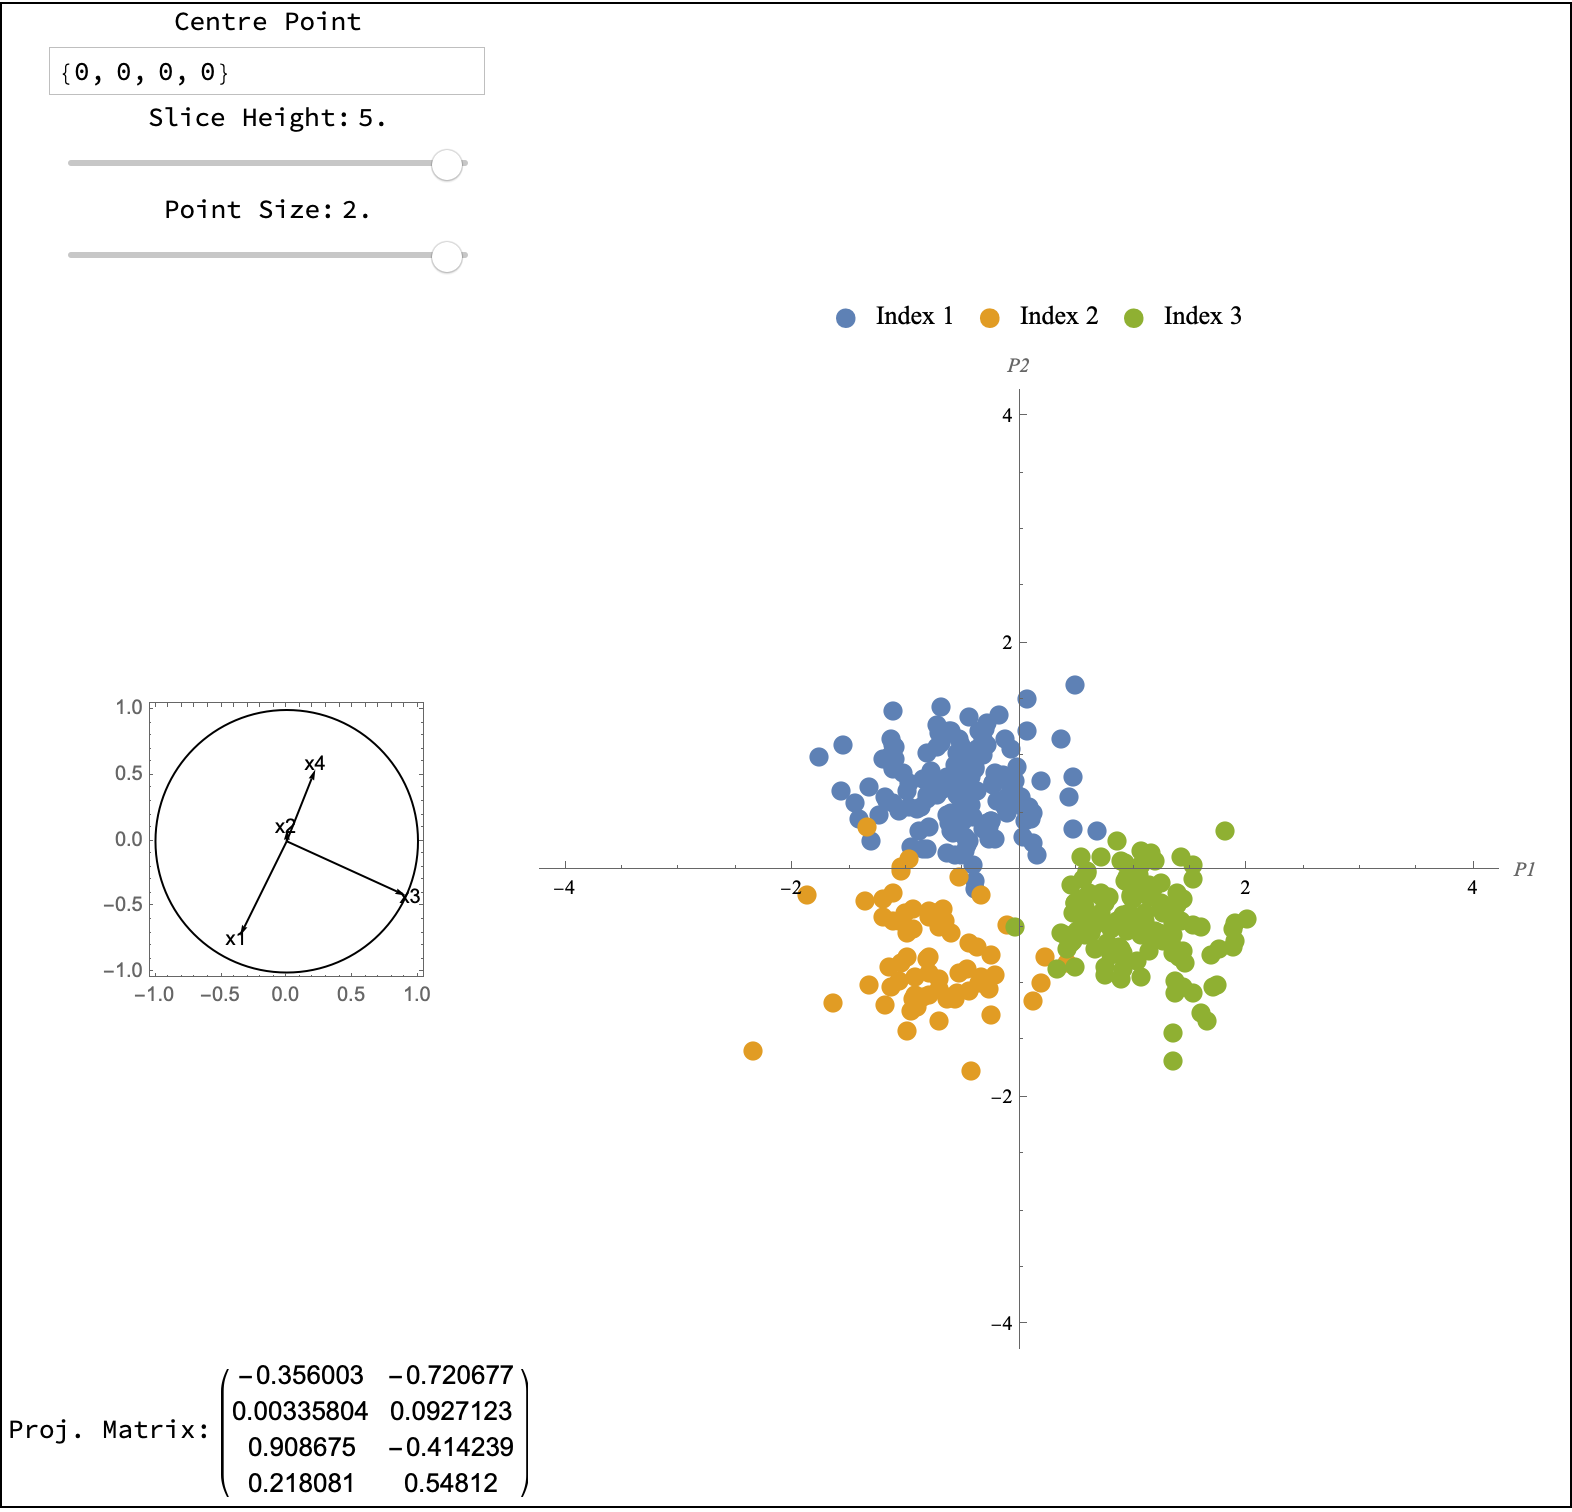
\includegraphics[width=0.32\textwidth]{figures/proj1_data.png}}
\caption{Projection identified using the manual tour, because it reveals an interesting structure in the predictions from the RF model (left). We can clearly see a block structure, while the LDA model (middle) produces linear boundaries. The three groups are nicely separated in this projection of the data (right)}.
\label{proj1}
\end{figure*}

\hypertarget{slicing-through-the-center}{%
\subsection{Slicing through the
center}\label{slicing-through-the-center}}

XXXX currently in the notebook \(A_1\) is called A5, and \(A_2\) is
called A6

We continue the investigation by now slicing orthogonally to the
projection \(A_1\). For both models we look at a thin (\(h=0.5\)) slice
through the center, \(S_1^0 = (0,0,0,0)\). At first we explore how
changing the projection, and thus the slice) away from \(A_1\) can help
with understanding the boundary better. For our example, notice that
\(A_1\) does not contain any contribution from the second variable
(\texttt{bd}), so we will first rotate this variable into the view.

Figure \ref{slice1} shows snapshots of the exploration. The rop row is
the initial projection (\(A_1\) and \(S_1^0\)), and the bottom row is a
later projection containing more of \texttt{bd} (call them \(A_2\) and
\(S_2^0\)). The columns correspond to the two models, with Rf on the
left and LDA on the right.

Both models have some overlap at the center, even for this thin slice
(\(S_1^0\)). The second slice (\(S_2^0\)) mostly resolves this overlap
and reveals the primary differences between the models. The boundary
between Adelie (blue) and Chinstrap (yellow) is very similar for both
models. The boundary between Chinstrap and Gentoo (green) is where they
differ.

The RF is almost straight in this view, as something we might expect
from a tree model where splitting occurs on single variables only.
However, it is straight in a combination of the second and third
variable (\texttt{bd} and \texttt{fl}). By examining the scatterplot
matrix, we can understand how this boundary was built: on each of
\texttt{bd} and \texttt{fl} it is possible to cut on a value where most
of the Gentoo penguins are different from the other two speciesfor any
tree, and likely only one is needed. Thus the forest construction is
providing a sample of trees that use one variable or the other variable
to split, producing the blocky boundary on the combination of the two.

In contrast, the LDA boundary has an oblique split between the two, and
roughly divides the space into three similarly sized areas. It is almost
like a textbook illustration of how LDA works for two variables (2D)
where by assuming the clusters have equal variance-covariance, it places
a boundary half-way between the group means.

\begin{figure*}[ht]
\centerline{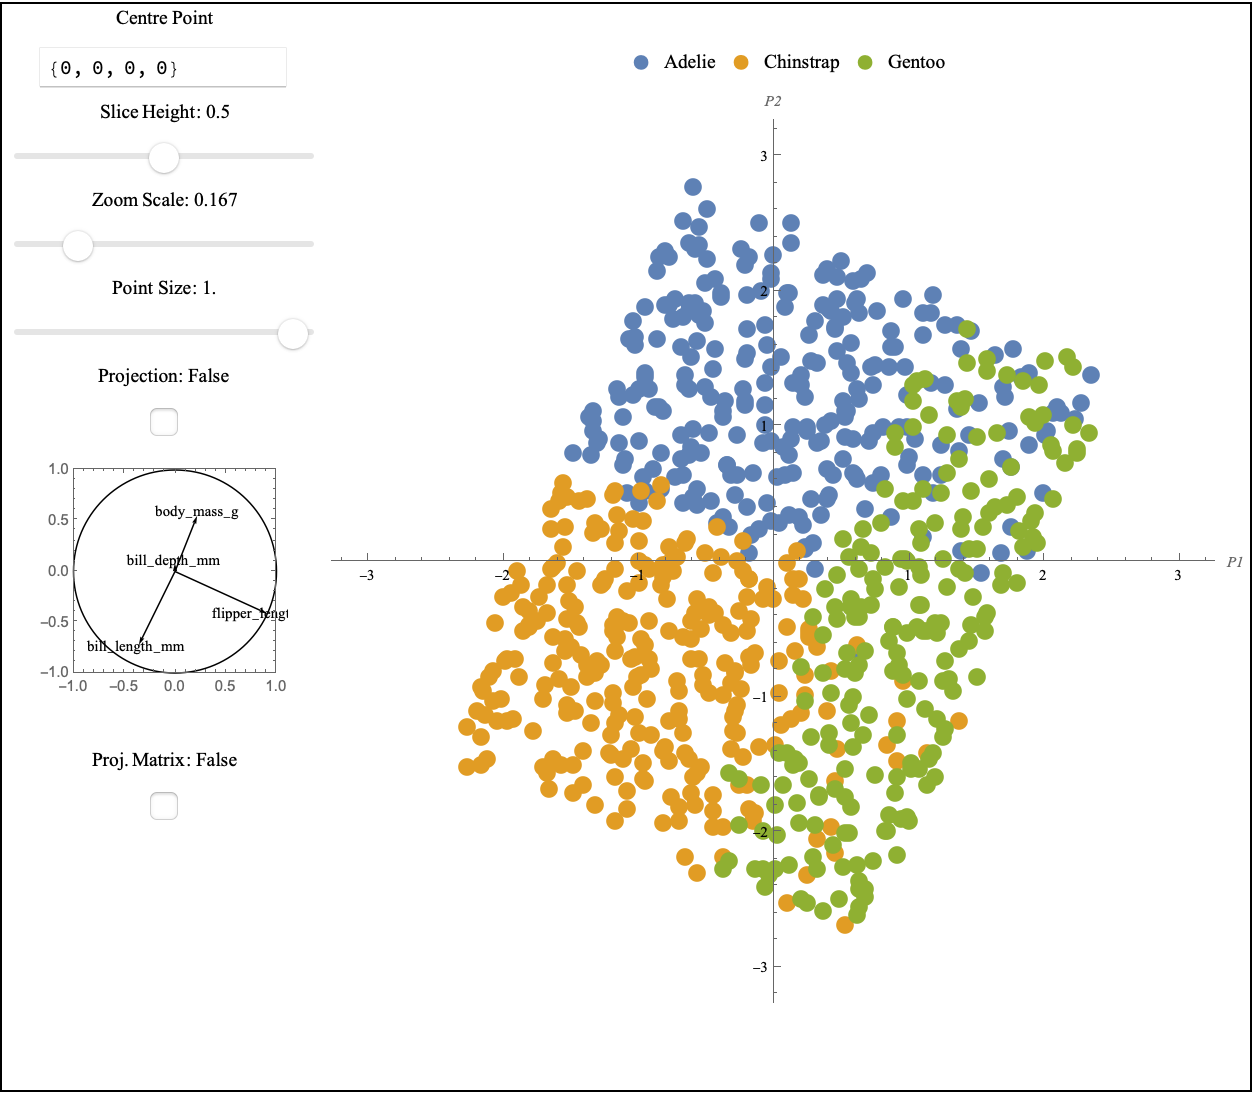
\includegraphics[width=0.45\textwidth]{figures/slice1_rf.png}
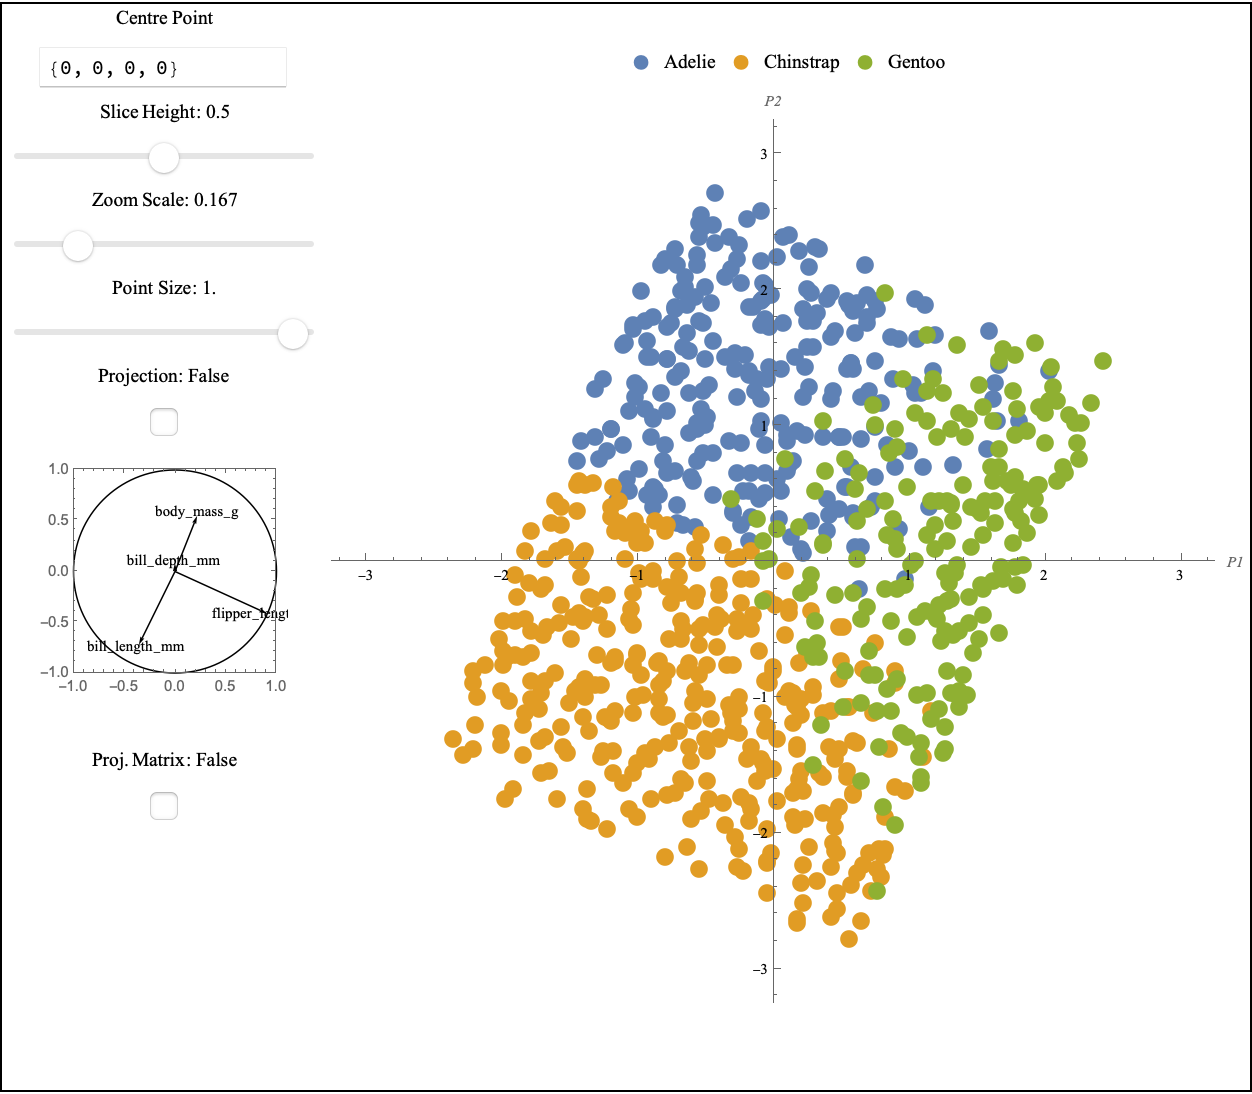
\includegraphics[width=0.45\textwidth]{figures/slice1_lda.png}}
\centerline{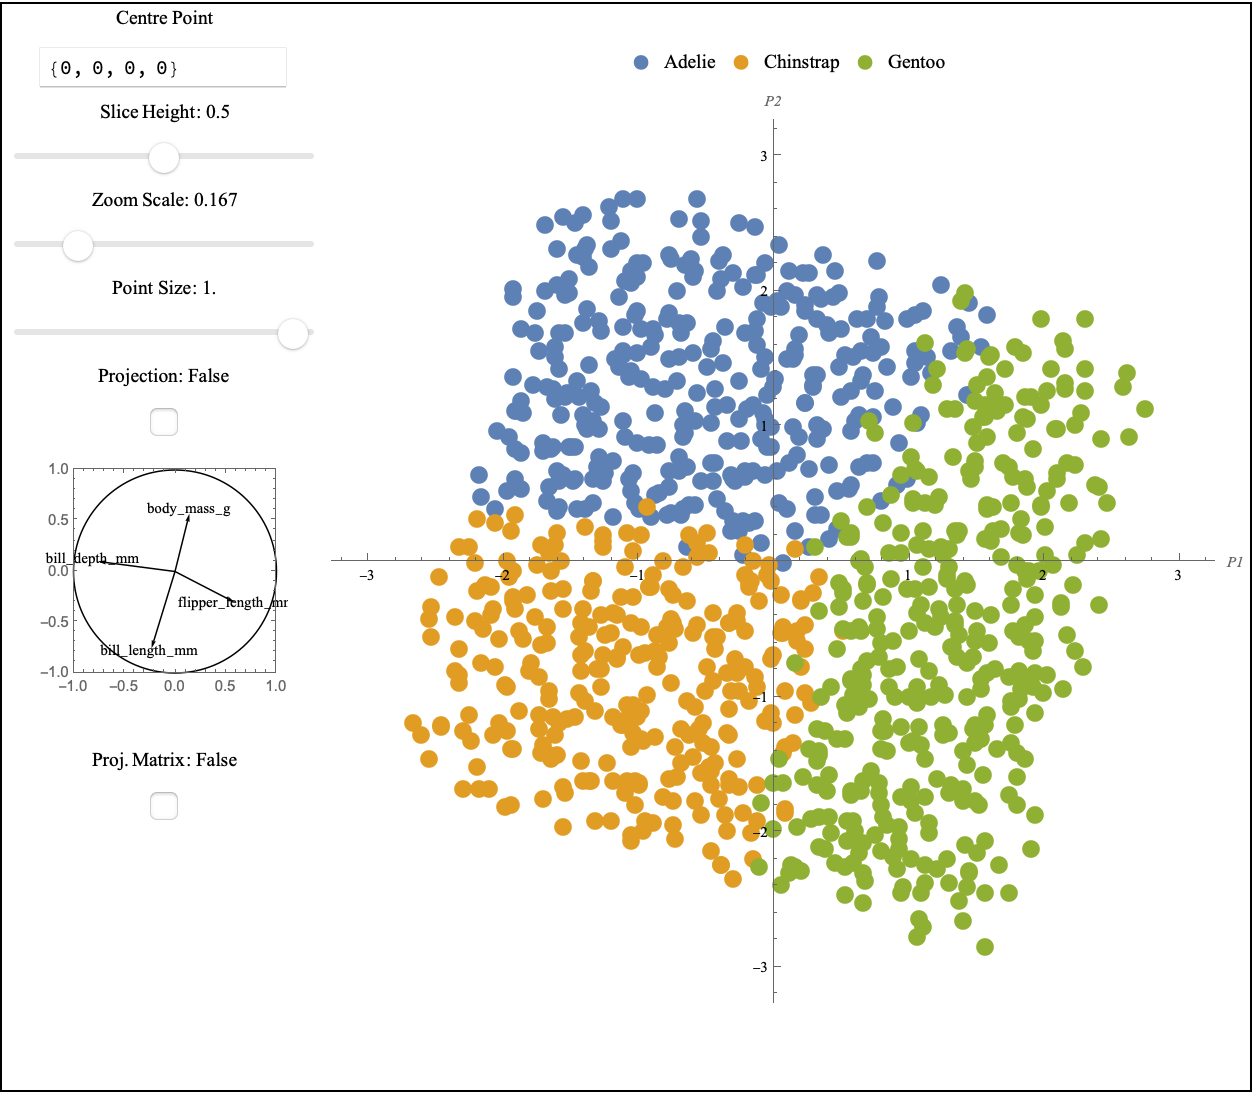
\includegraphics[width=0.45\textwidth]{figures/slice2_rf.png}
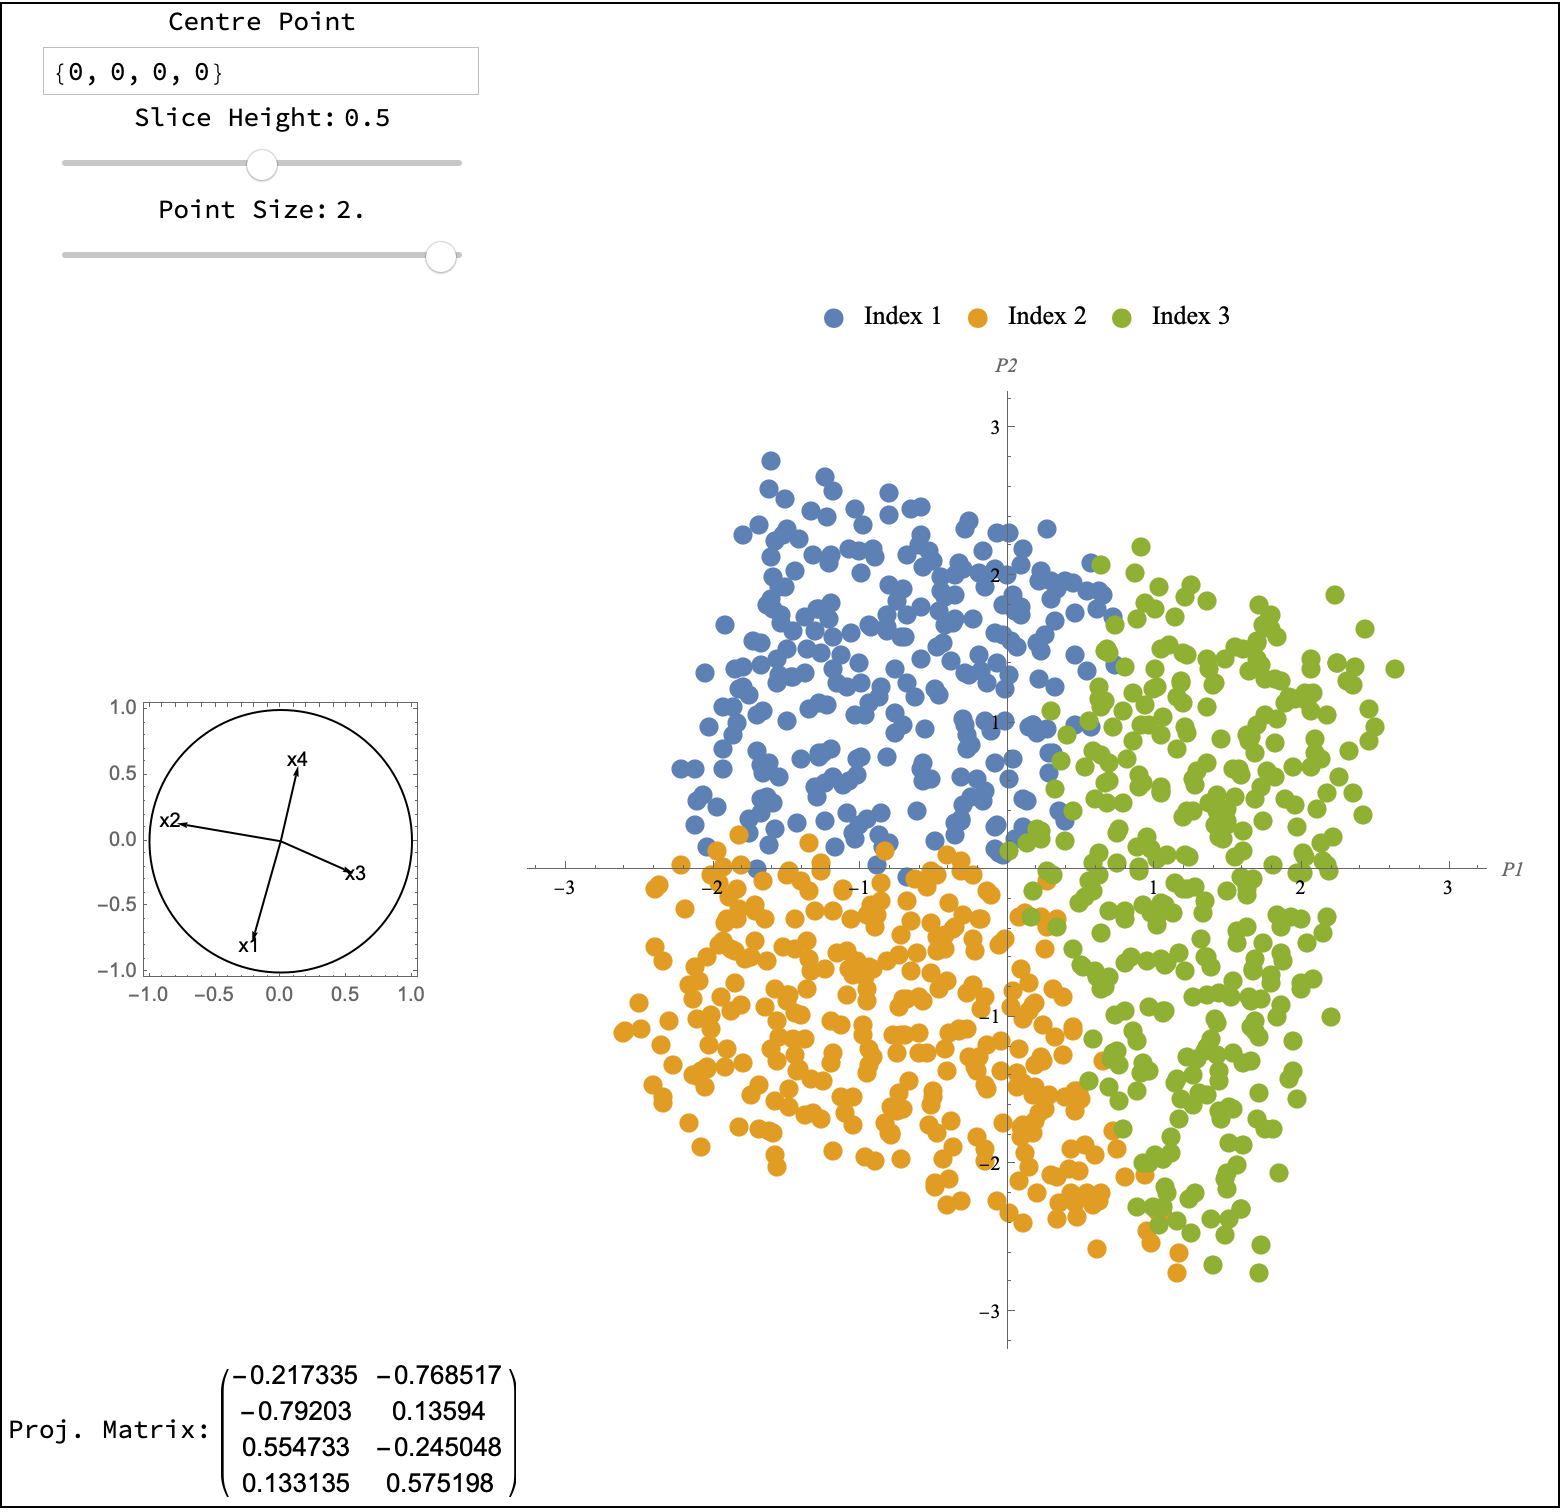
\includegraphics[width=0.45\textwidth]{figures/slice2_lda.png}}
\caption{Comparing slices based on two projections $A_1$ (top row) and $A_2$ (bottom row), for the two models RF (left) and LDA (right). With $A_1$ we see two groups overlap (green - Gentoo with yellow - Chinstrap), while the rotation to $A_2$ results in clear boundaries inside the slice. The boundary between Adelie (blue) and Chinstrap (yellow) is similar for both models but very different between Chinstrap and Gentoo (green).}
\label{slice1}
\end{figure*}

\begin{figure*}[ht]
\centerline{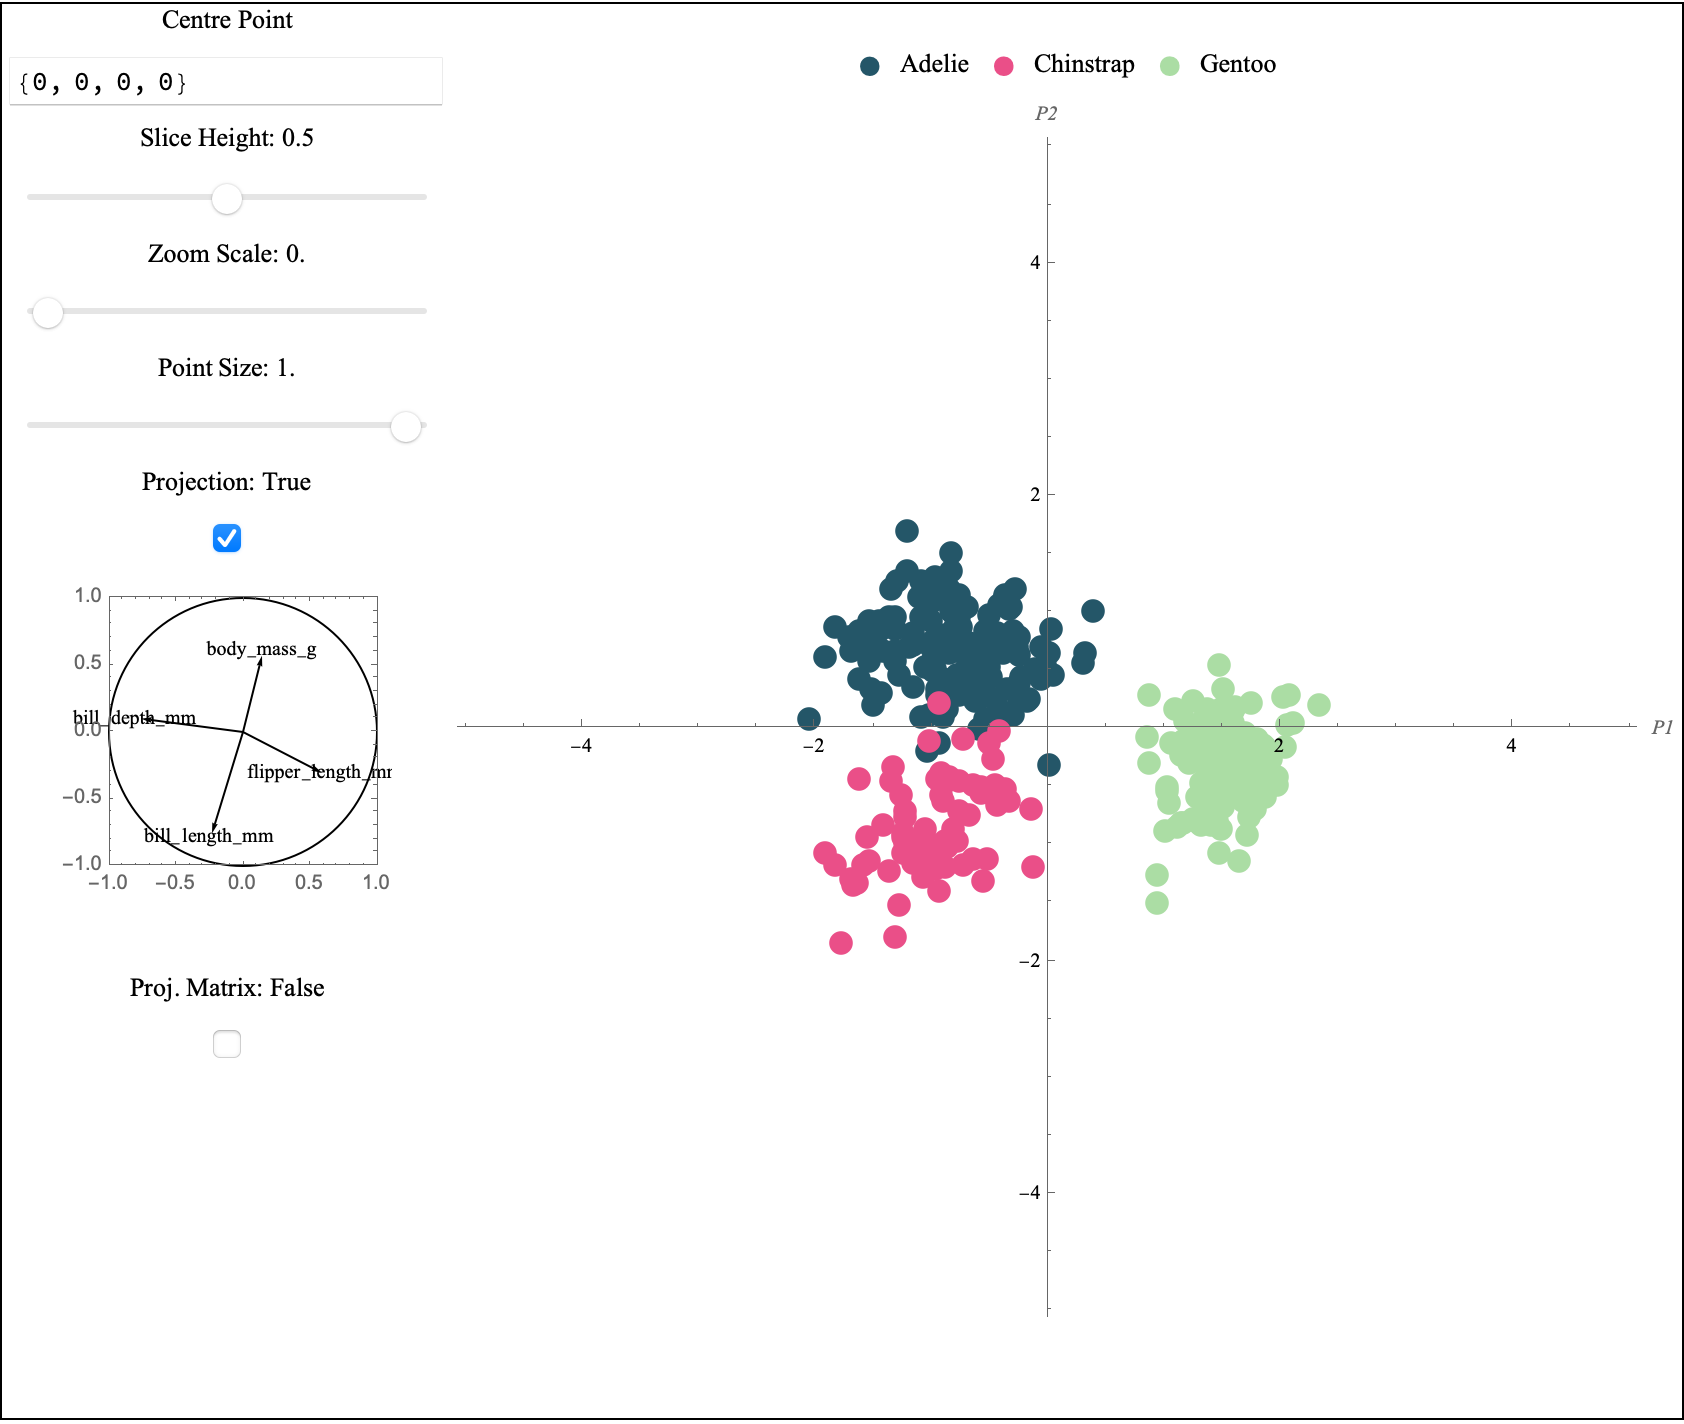
\includegraphics[width=0.45\textwidth]{figures/proj2_data.png}}
\caption{Projection of the data based on $A_2$. Compared to projecting onto $A_1$ we see that the green observations (Gentoo) are more separated from the other two species.}
\label{proj2}
\end{figure*}

Finally, to determine which model does the boundaries better, compare
them with the \(A_2\) projection of the data (Figure \ref{proj2}).
Gentoo is more separated from the other two in this projection, and one
can imagine that the trees in the forest has greedily grasped any one of
many places to make a split to separate the group. It might be argued
though the that RF boundary is cut too close to the Chinstrap species,
and might lead to some unnecessary misclassification with new data. The
LDA boundary is better placed for all species.

\hypertarget{shifting-the-slice-center}{%
\subsection{Shifting the slice center}\label{shifting-the-slice-center}}

We have seen that starting from \(A_1\) using the manual controls to
change the contribution of the second variable we could find a clear
separation boundary indicating the relation between this variable (bill
depth) and the Gentoo penguin species. Instead of rotating to a
different projection, we might also change the view by moving the slice
along one axis in the 4D space. Here we will continue our exploration of
the dependence on \texttt{bd} and move the slice defined by \(A_1\),
\(S_1^c\) to either large positive or negative values
(\(c_{bd} = \pm 1.5\) after centering and scaling). We will label these
slices as \(S_1^{\pm}\). Here we will also look at slices of the
observed data points, using a thicker slice (\(h=1.5\)) to capture
enough points in a given view.

We start by a comparison of the two models and the data distribution in
\(S_1^{+}\), thus the slice is localized towards high values of bill
depth in Figure \ref{slice1p}. We can see that all three slices (the two
models and the data) contain almost no points from the third class
(green, Gentoo), and that the decision boundary between the two models
is very similar.

\begin{figure*}[ht]
\centerline{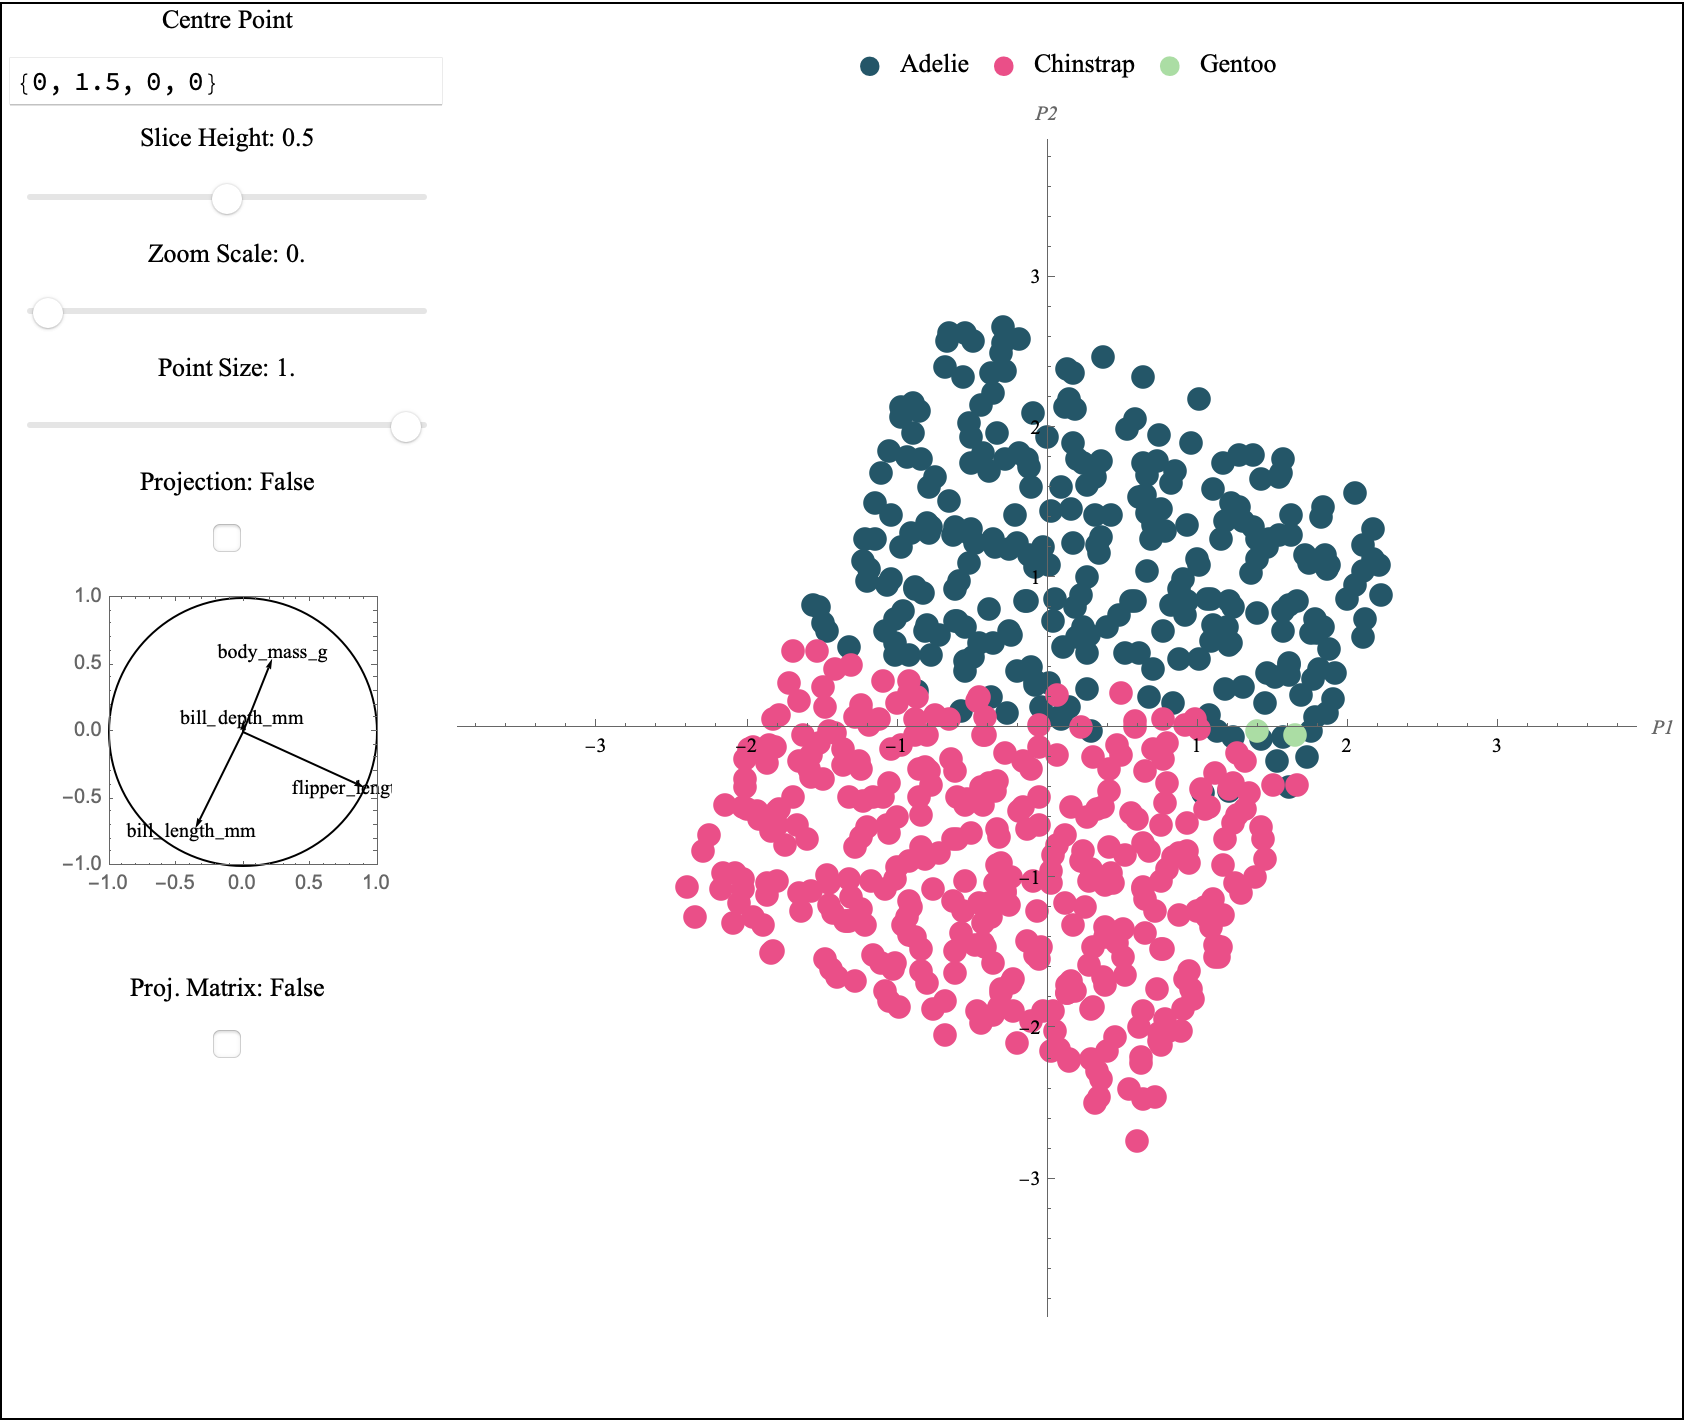
\includegraphics[width=0.32\textwidth]{figures/slice1_p_rf.png}
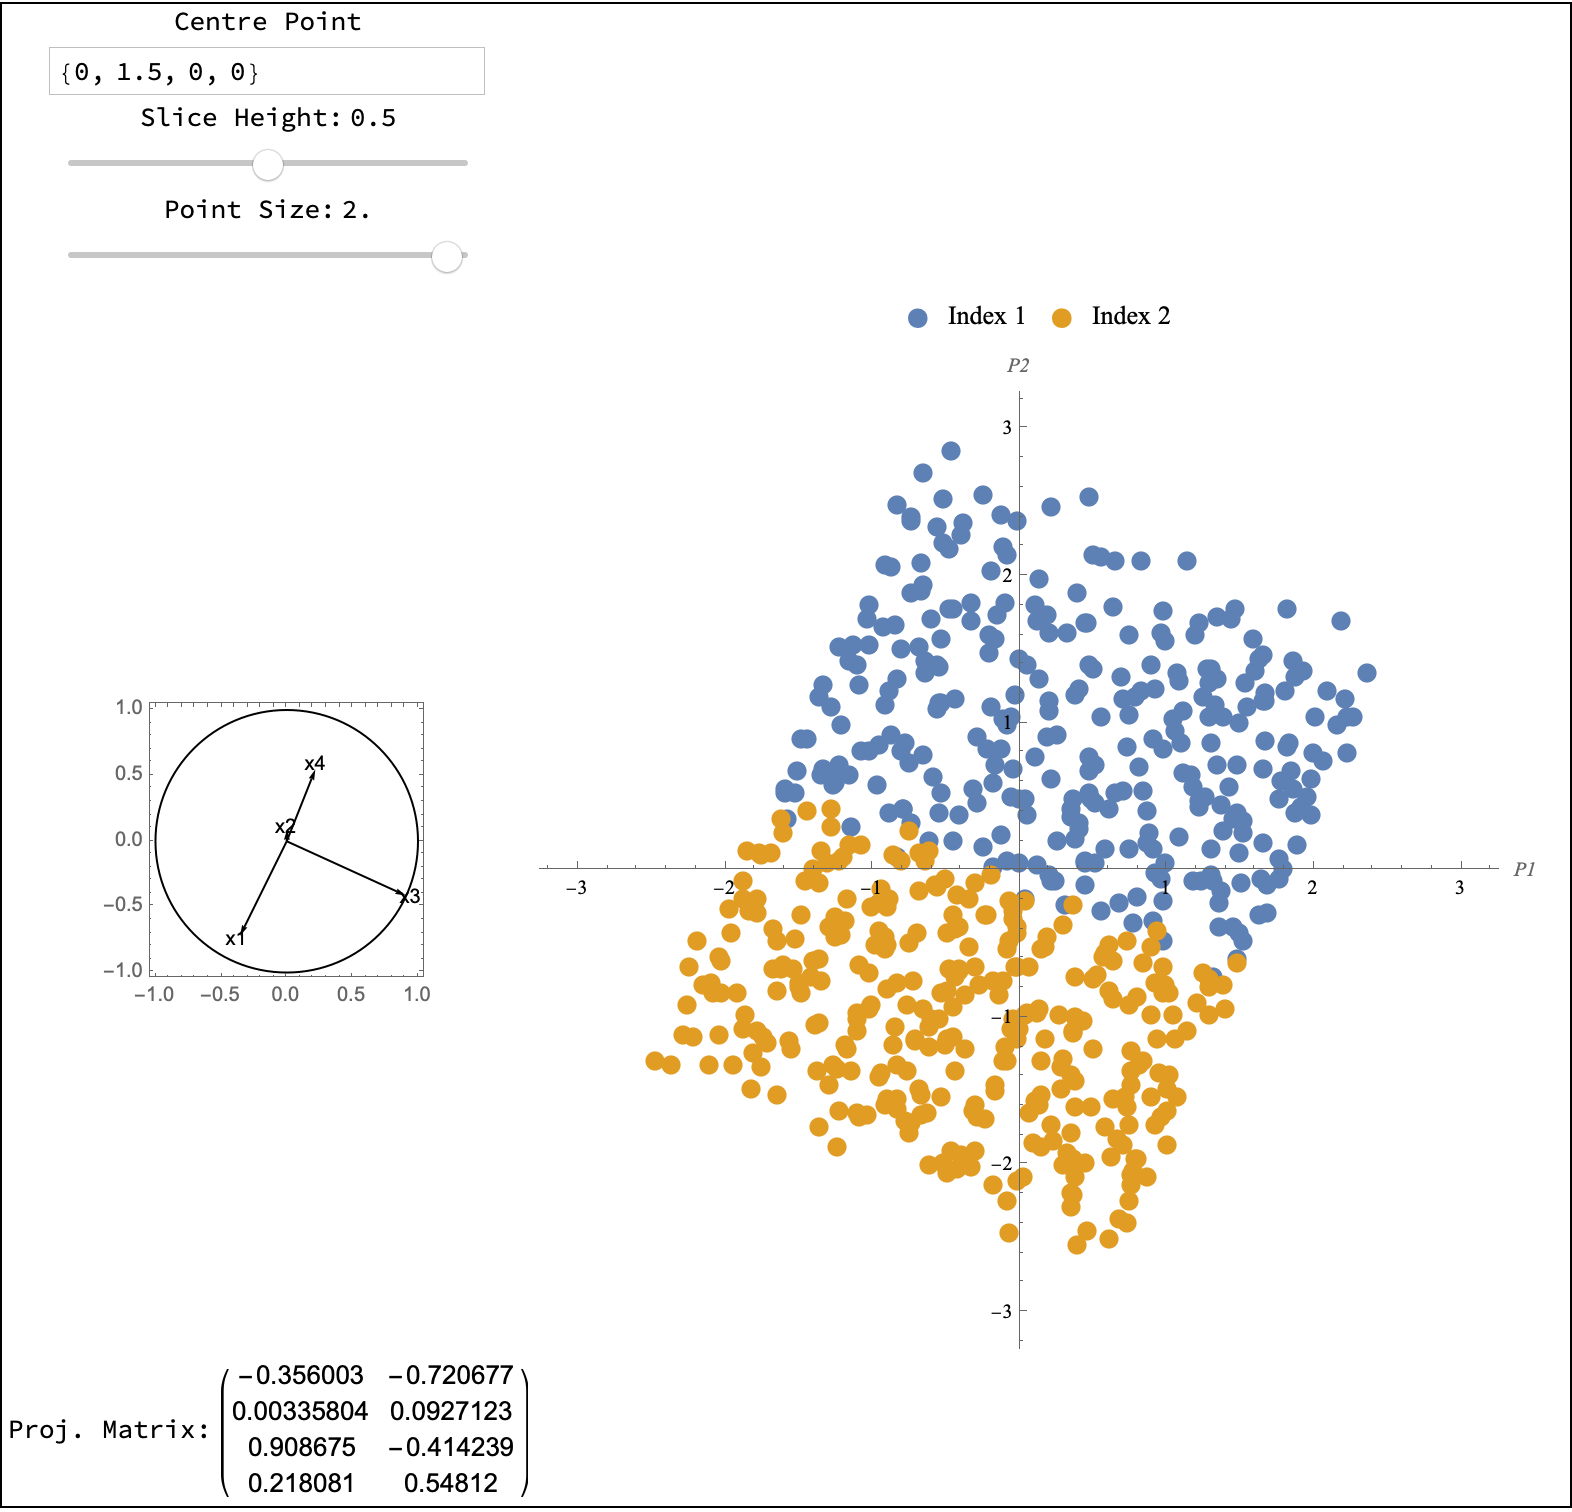
\includegraphics[width=0.32\textwidth]{figures/slice1_p_lda.png}
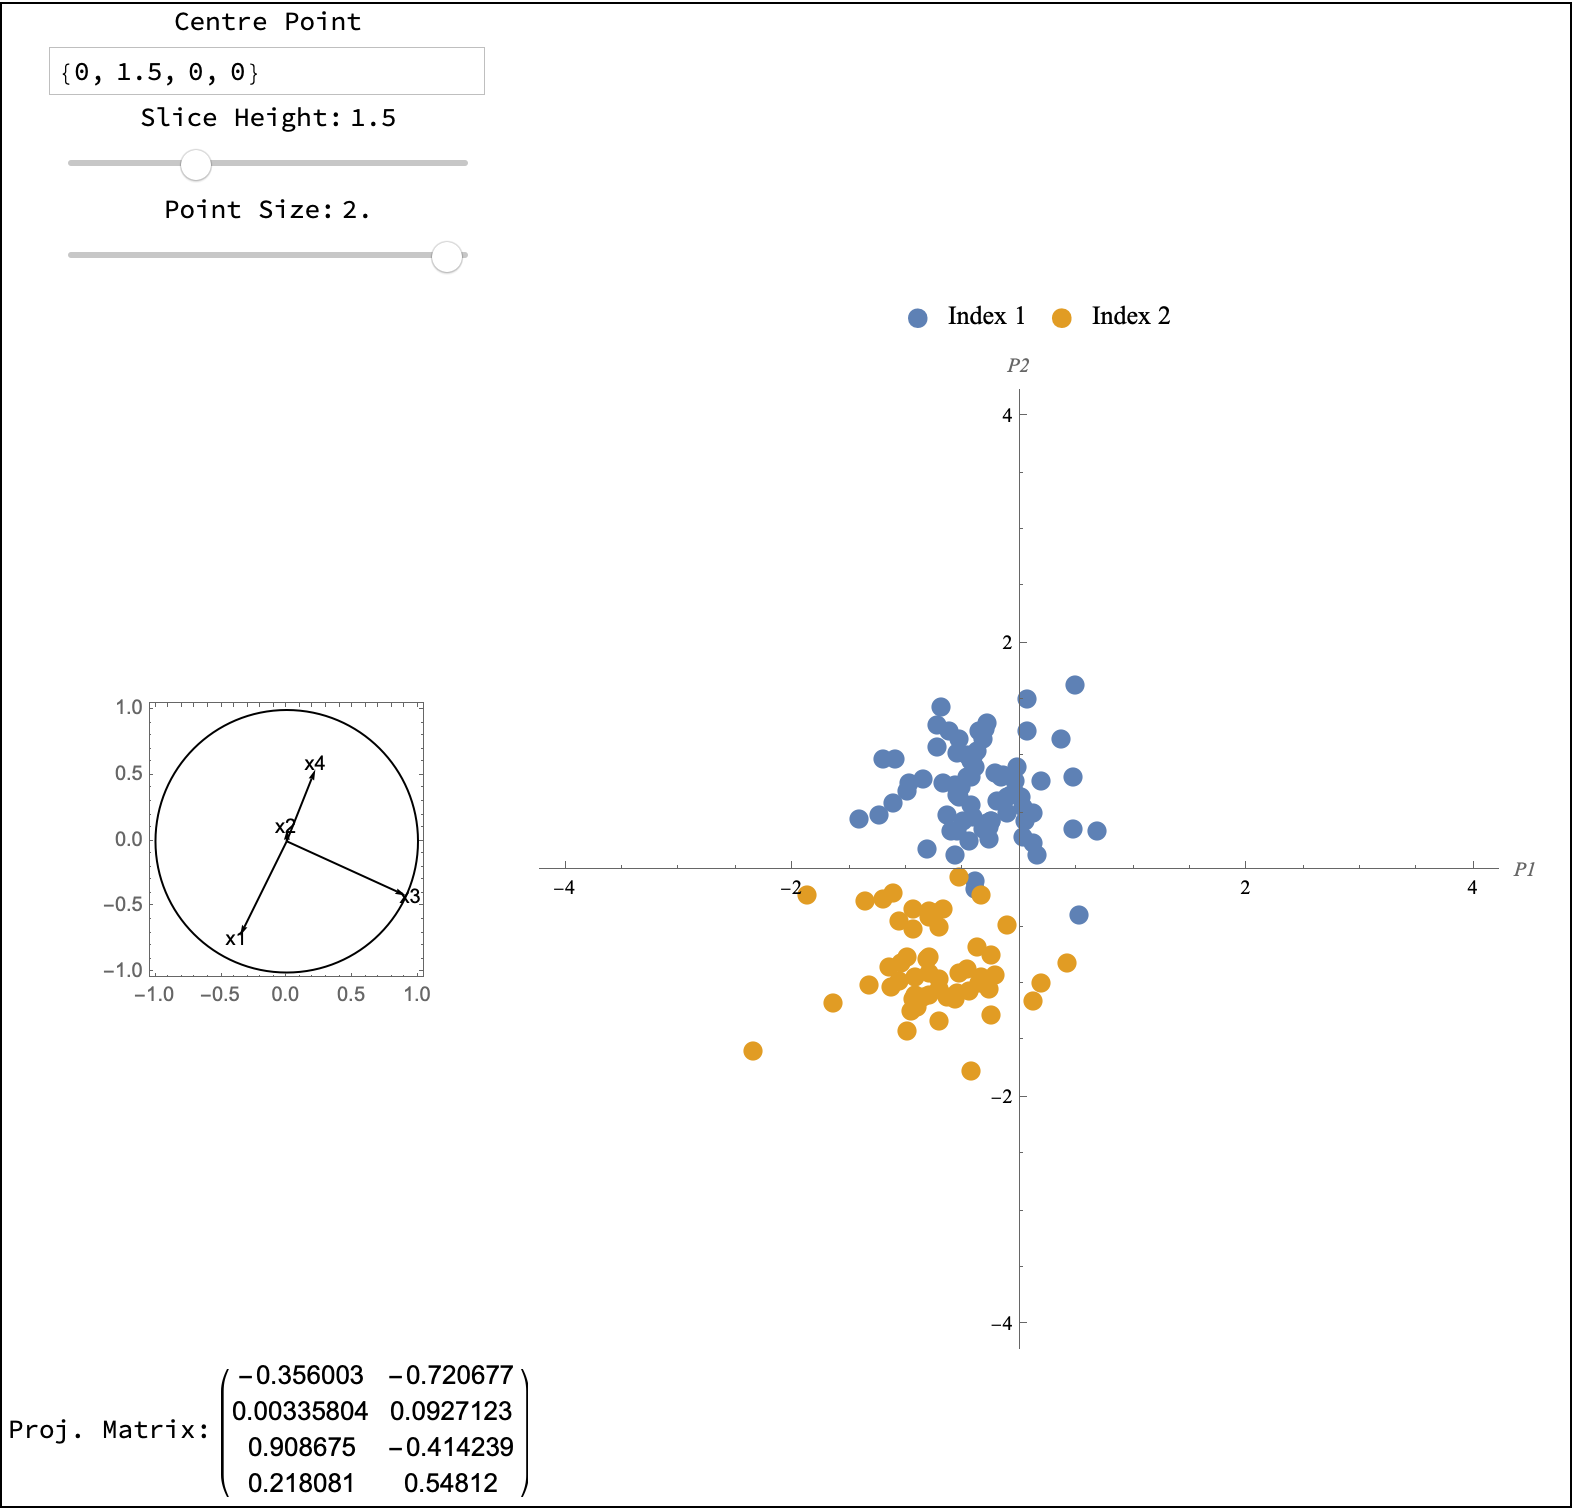
\includegraphics[width=0.32\textwidth]{figures/slice1_p_data.png}}
\caption{Shifting the slice center in the positive direction of bill depth produces regions that have no Gentoo (green). The two models have similar boundaries except that the RF is more of a step function.}
\label{slice1p}
\end{figure*}

\begin{figure*}[ht]
\centerline{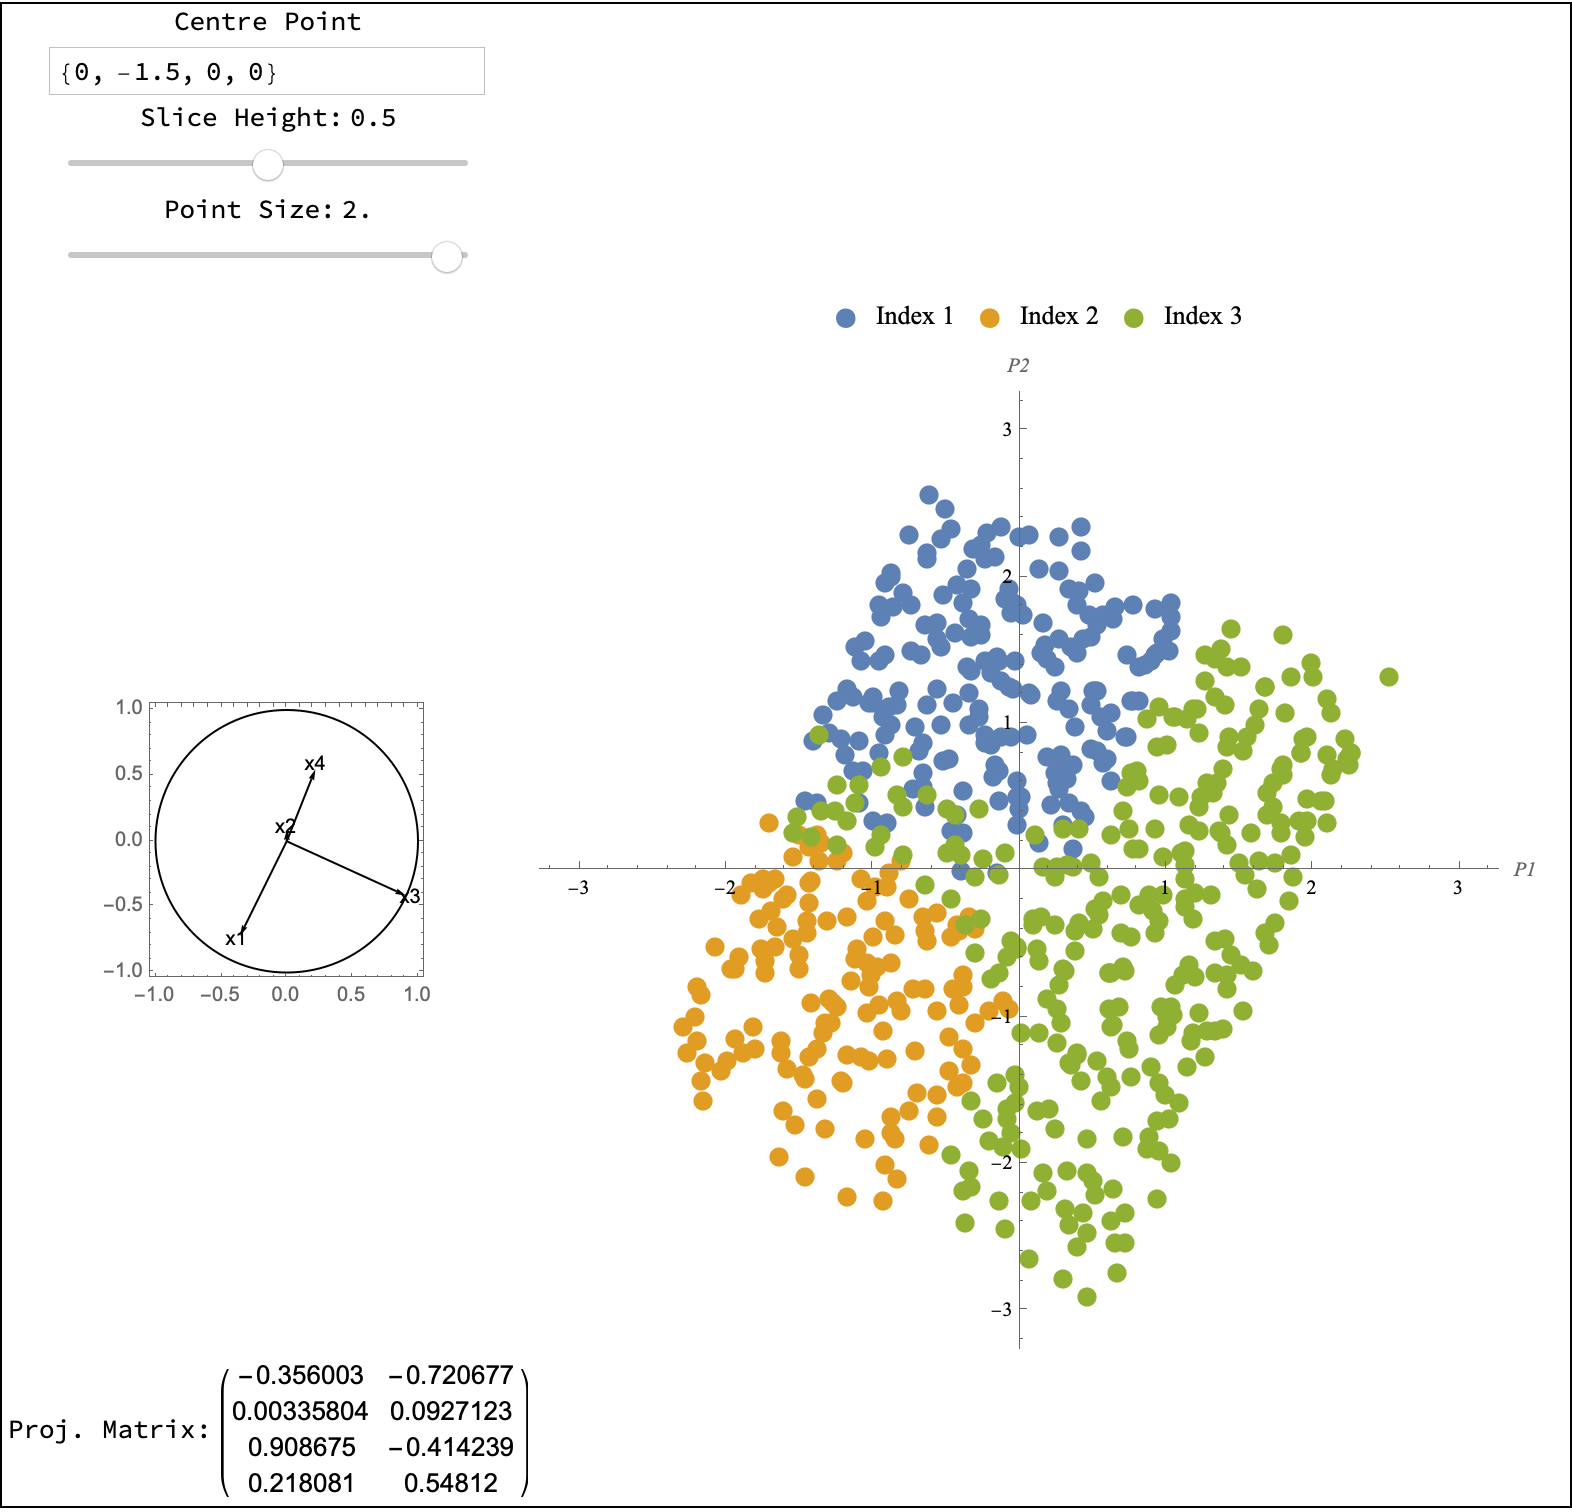
\includegraphics[width=0.32\textwidth]{figures/slice1_m_rf.png}
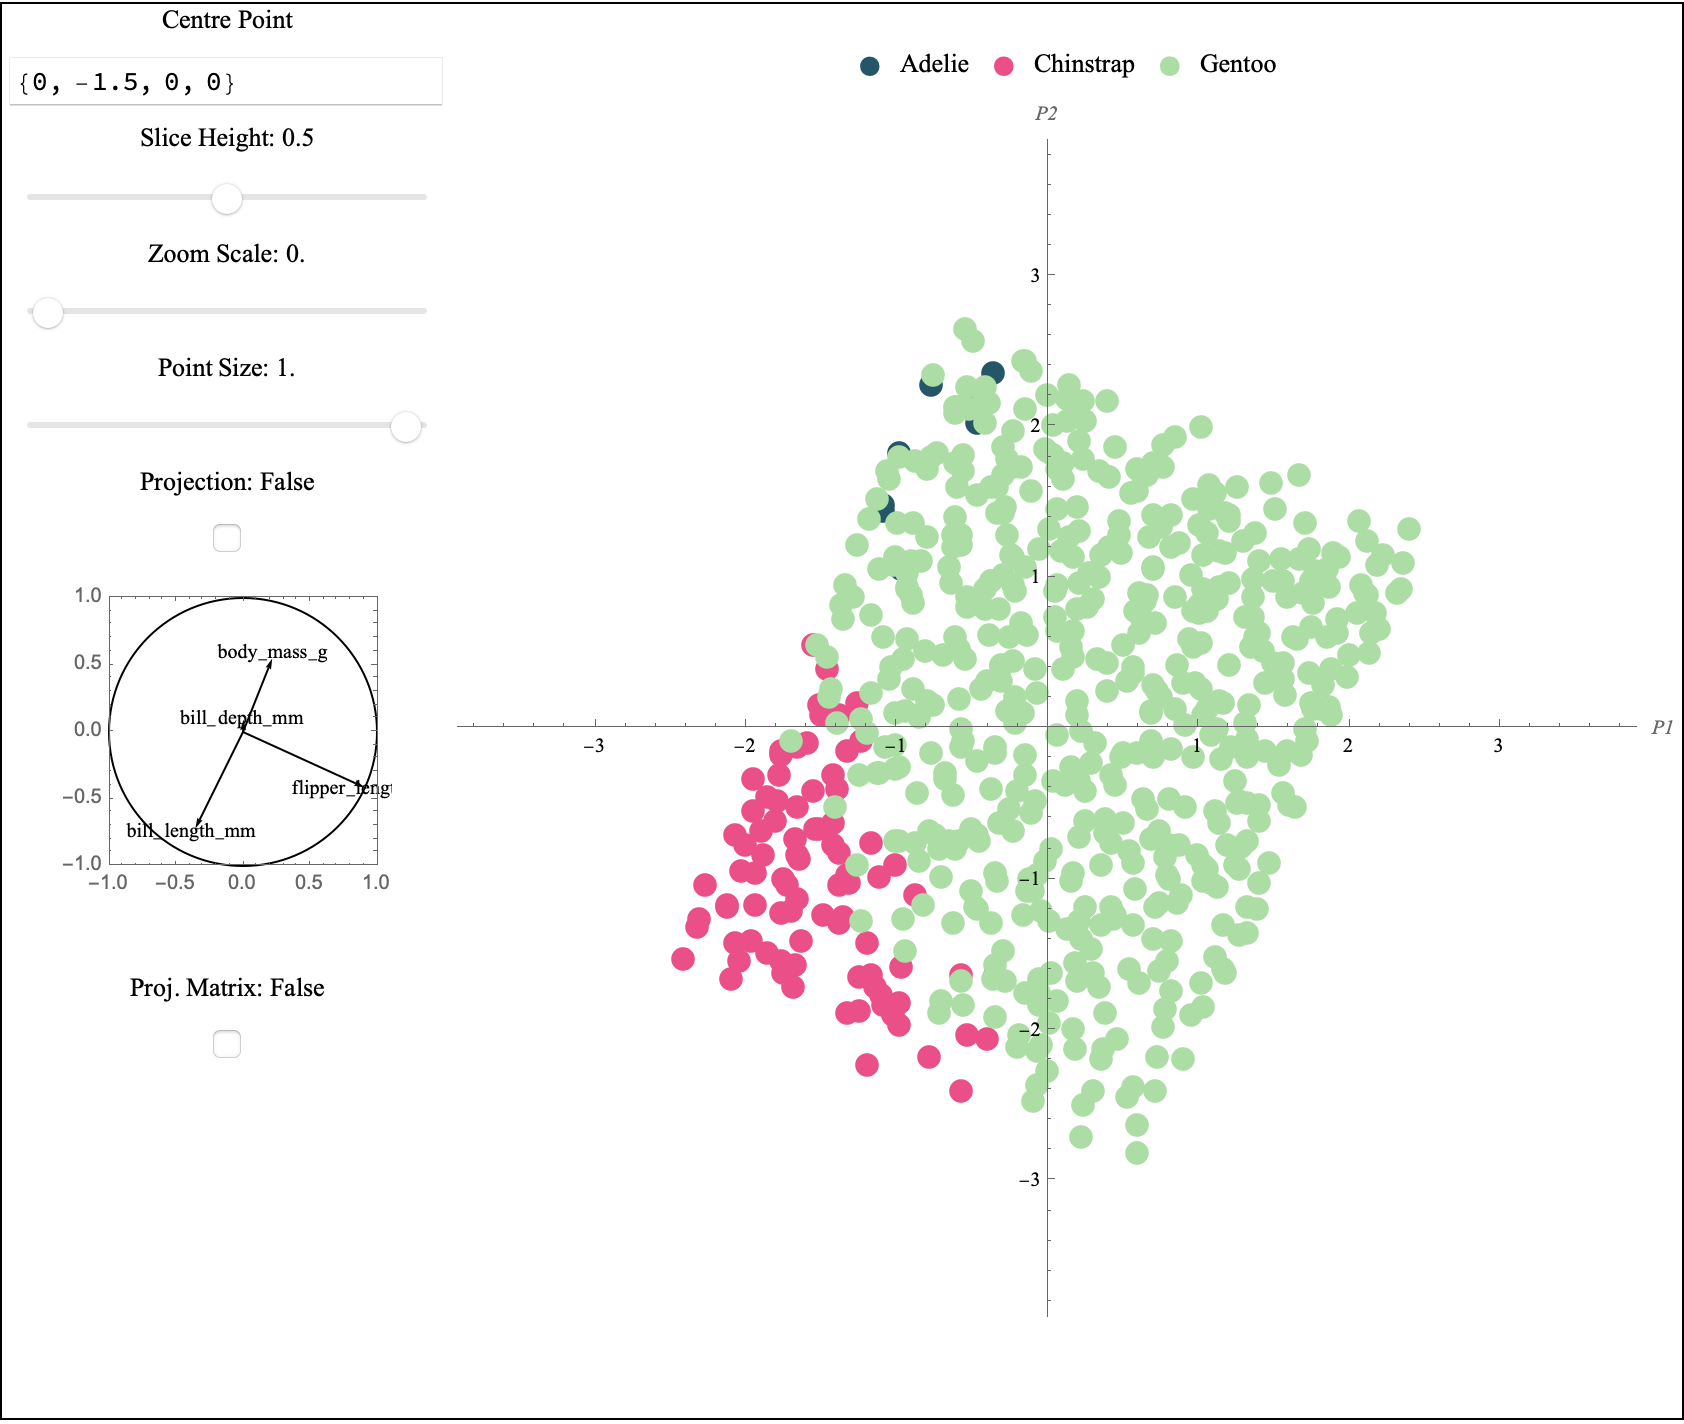
\includegraphics[width=0.32\textwidth]{figures/slice1_m_lda.png}
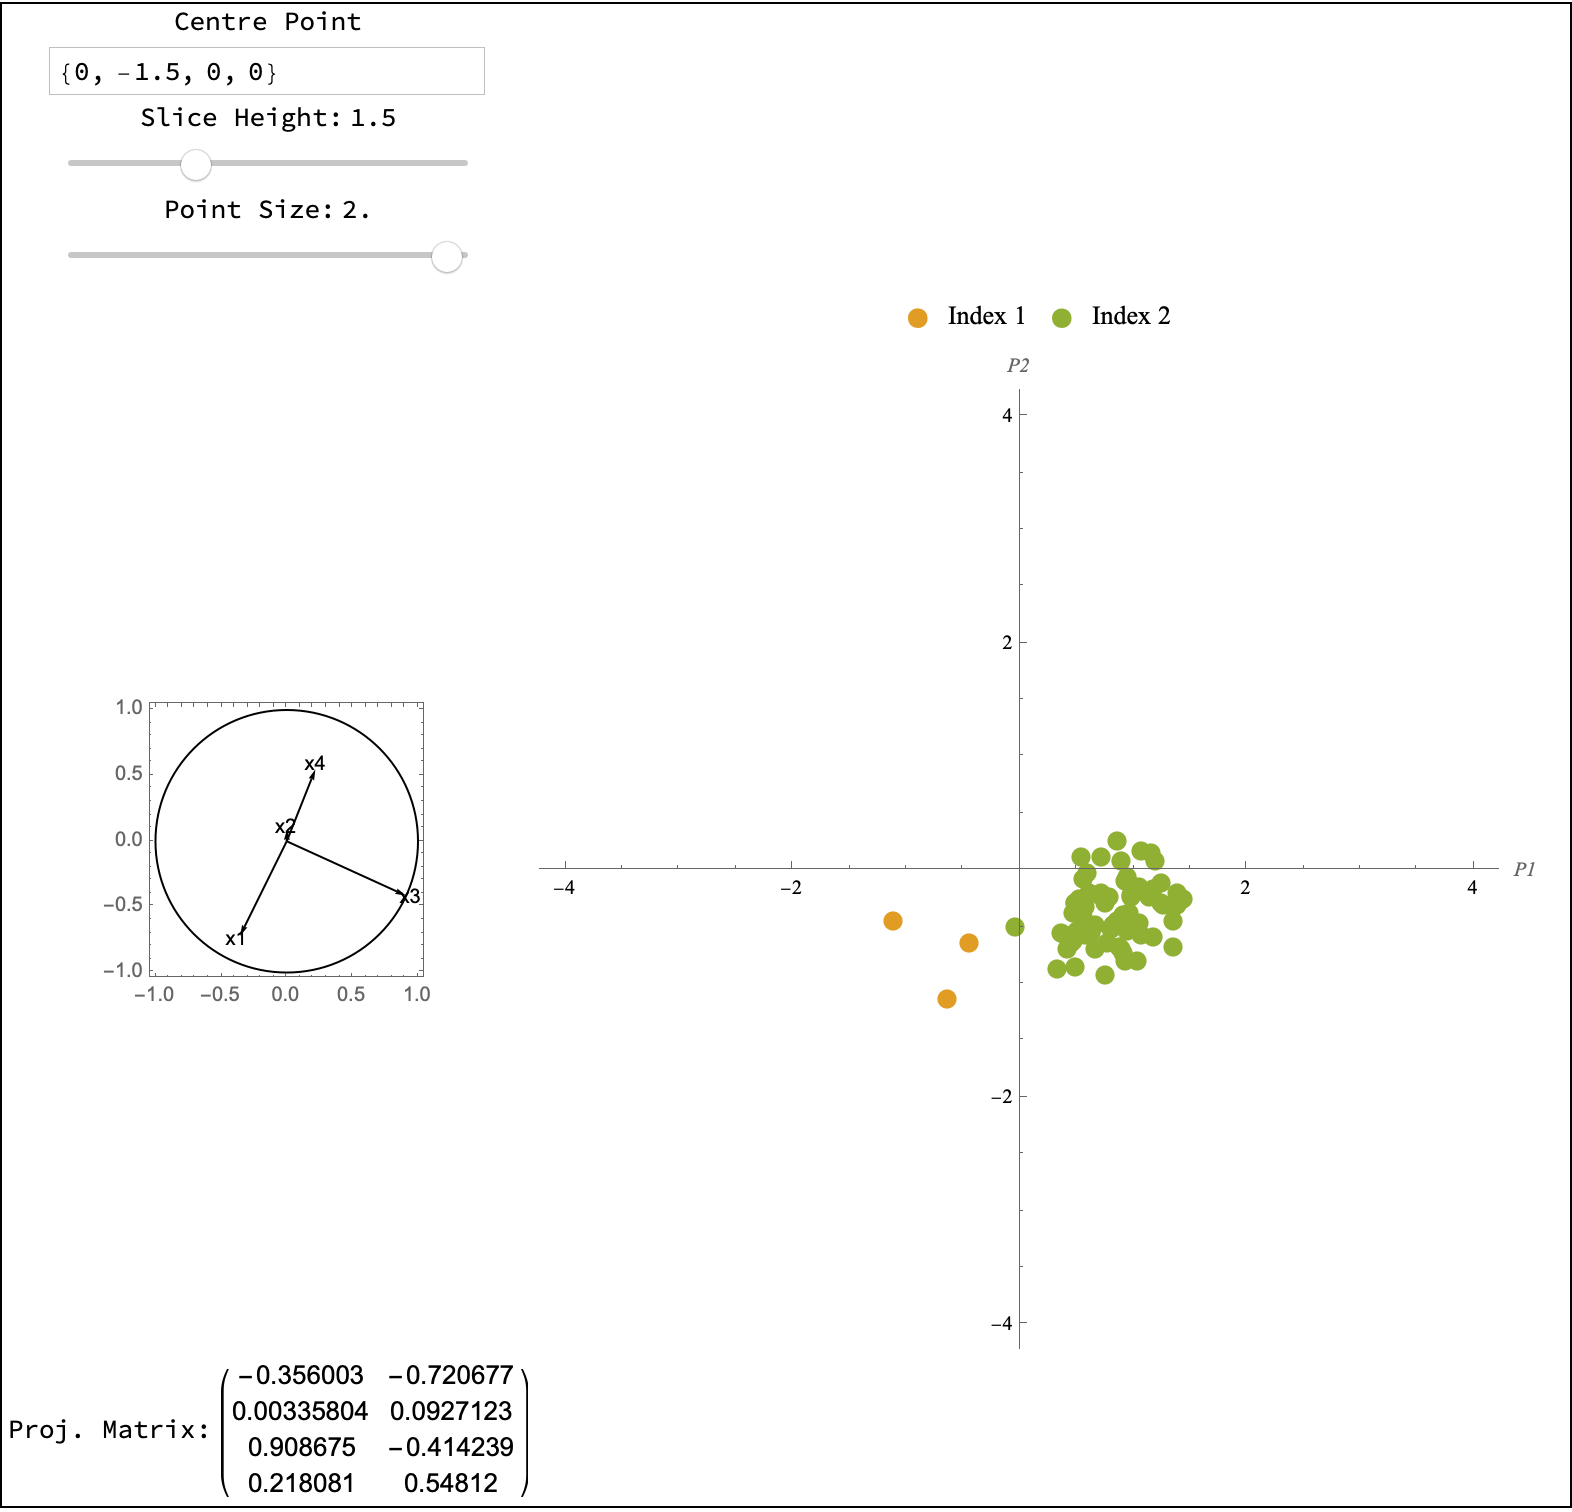
\includegraphics[width=0.32\textwidth]{figures/slice1_m_data.png}}
\caption{Shifting the slice center in the negative direction of bill depth produces regions that are mostly Gentoo (green). The two models have very different boundaries: the nonlinear potential of RF can be seen here where still some subspaces would predict to be Adelie and Chinstrap.}
\label{slice1m}
\end{figure*}

A more interesting comparison is found for \(S_1^{-}\), thus the slice
localized towards low values of bill depth, shown in Figure
\ref{slice1m}. The RF model (left) predicts all three species within
this slice, with an interesting boundary for the third class (green,
Gentoo). On the other hand the LDA model (middle) predominantly predicts
the third class within the slice, this appears to be enforced through
the linear structure of the model. Looking finally at the thick slice
through the data we see that there are primarily observations from this
class within the slice we can conclude that the two models have filled
in the ``empty'' space (where we do not have any training observations)
in very different ways and according to what we might expect given the
model structure.

Finally it is interesting to compare the slice views to the projection
of the models seen in Fig. \ref{proj1} to better understand how the
boundaries change along the \texttt{bd} direction and where the
differences in the projections come from.

\hypertarget{sec:implementation}{%
\section{Software}\label{sec:implementation}}

XXX copied from the slicing part to be weaved in below:

The current implementation allows the user to individually enter the
components of the vector defining the center point, and updates the
display by jumping to the new slice.

The current implementation contains a switch to change between the slice
view and the projected view of the data, while keeping all other
settings fixed.

\hypertarget{mathematica-notebook}{%
\subsection{Mathematica notebook}\label{mathematica-notebook}}

\begin{itemize}
\tightlist
\item
  \textbf{Why is this a good sandbox}
\item
  \textbf{Explain the functionality available in the notebooks}
\end{itemize}

Mathematica provides much utility and versatility, such as inbuilt data
visualisation, data manipulation and analysis, dynamic functionality,
and symbolic and numeric computation. Most of this inbuilt functionality
is quite user-friendly and can be found in the Mathematica
documentation; typically, numerous examples are provided within the
documentation, and some possible issues are outlined there. Also, it is
relatively simple to create dynamic objects via the inbuilt commands
Manipulate or DynamicModule. Control objects, such as sliders, locator
panes, and input fields, can then be used on dynamic variables, and when
there is a change in the dynamic variable the dynamic objects which
contain that dynamic variable will be updated. This is the essential
ingredient for this implementation of the manual tour. However, it can
be hard to alter the behaviour of the control objects such as setting
the 1D slider on a different scale (Slider increments add 10 points into
the slice rather than increasing the slice height by 0.1 for example).
\{\textcolor{red}Alex, is this still true with the controls you are
using now?\}

The examples presented in the penguins' notebooks all utilise our
primary new function, SliceDynamic. This function typically accepts
grouped data in the form of a matrix where the second last column
details the name of the group and the last column details the group
index. After specifying the initial slice height and the slice range,
the user is then presented with an interactive display in which the
control objects appear on the left and the slice visulisation appears on
the right. The user can change the orientation of the slice via the
locator pane, which changes the projection matrix; a slider controls the
slice height; and there is an input field, which changes the slice
centre. The user can also change the appearance of the plot by zooming
into the center or changing the point size with sliders provided. The
current projection can be displayed to contrast it with the slice by
ticking a box. The explicit projection matrix can be displayed via
another checkbox. The Slice Tour* notebooks include the additional
functions: ProjectionPlot, Projected2DSliderPlot, and
VisualiseSliceDyanmic. ProjectionPlot is very similar to SliceDynamic,
except it only displays projections and VisualiseSliceDynamic allows you
to discern which points exist inside the slice and outside it. However,
ProjectedLocatorPlot displays the interactive slightly differently.
Several locator panes are displayed above the plot and each one
corresponds to a row in the projection matrix but behaves the same as
ProjectionPlot. \{\textcolor{blue}(this may be easier to implement in
another language (?) )\}

\hypertarget{extensions-to-the-r-package-tourr}{%
\subsection{\texorpdfstring{Extensions to the R package
\texttt{tourr}}{Extensions to the R package tourr}}\label{extensions-to-the-r-package-tourr}}

The \citet{tourr} package provides numerous types of tours. An
additional function has been constructed that will generate a sequence
of projections that will decrease the coordinates for \(V_m\) to
\(\boldsymbol{0}\) and back to the original values. It is applicable for
any projection dimension, \(d\).

Changing slice center

\hypertarget{desirable-interactivity}{%
\subsection{Desirable interactivity}\label{desirable-interactivity}}

Potential adjustments for future work include a better visualization of
the current center point, potentially with interactive graphics to move
the slice similar to how the manual tour was implemented here. An
alternative would be a step-wise shift of the slice towards the new
center point to get a better understanding of the distribution along the
selected direction.

\hypertarget{sec:discussion}{%
\section{Discussion}\label{sec:discussion}}

Recap contribution

Other applications

Where else might it be useful to use mathematica

Maybe extensions for slicing

\hypertarget{acknowledgements}{%
\section*{Acknowledgements}\label{acknowledgements}}
\addcontentsline{toc}{section}{Acknowledgements}

The authors gratefully acknowledge the support of the Australian
Research Council and the ResearchFirst undergraduate research program at
Monash University. The paper was written in \texttt{rmarkdown}
\citep{rmarkdown} using \texttt{knitr} \citep{knitr}. The scatterplot
matrix of the penguins data was produced by the GGally \citep{GGally}
package built on ggplot2 \citep{ggplot2} graphics. We thank the
Institute of Statistics, BOKU, for their hospitality while part of this
work was conducted.

\hypertarget{supplementary-material}{%
\section*{Supplementary material}\label{supplementary-material}}
\addcontentsline{toc}{section}{Supplementary material}

The source material and animated gifs for this paper are available at

Mathematica notebook

Appendix

\bibliographystyle{tfcad}
\bibliography{biblio.bib}





\end{document}
